% =====================================================================
%  Parcial I — Paralelismo en Acción: Juego de la Vida paralelizado
%  750023C Infraestructuras Paralelas y Distribuidas — Univalle 2026-2
%
%  Compilar:  python informe/generar_datos.py   (cifras desde resultados/)
%             cd informe && latexmk -pdf informe.tex
%  También compila en Overleaf (subir la carpeta informe/ y resultados/figuras/).
%


% =====================================================================
\documentclass[11pt,a4paper]{article}

\usepackage[spanish,es-tabla,es-nodecimaldot]{babel}
\usepackage[T1]{fontenc}
\usepackage[utf8]{inputenc}
\usepackage{lmodern}
\usepackage{microtype}
\usepackage[margin=2.4cm]{geometry}
\usepackage{graphicx}
\usepackage{booktabs,multirow,tabularx,array}
\usepackage{amsmath}
\usepackage{xcolor}
\usepackage{listings}
\usepackage{caption,subcaption}
\usepackage{enumitem}
\usepackage{float}
\usepackage{tikz}
\usetikzlibrary{arrows.meta,positioning,decorations.pathreplacing,calc,fit}
\usepackage{fancyhdr}
\usepackage[hidelinks]{hyperref}

\graphicspath{{figuras/}{../resultados/figuras/}}
% Generado por informe/generar_datos.py — no editar a mano
\newif\ifborrador\borradorfalse
\expandafter\def\csname dato@cpu\endcsname{Intel Core i5-12450H (4 núcleos P con HT + 4 núcleos E)}
\expandafter\def\csname dato@nucleos-log\endcsname{12}
\expandafter\def\csname dato@nucleos-fis\endcsname{8}
\expandafter\def\csname dato@sistema\endcsname{Linux 7.2.9-arch1-1}
\expandafter\def\csname dato@python\endcsname{3.12.15}
\expandafter\def\csname dato@numpy\endcsname{2.5.4}
\expandafter\def\csname dato@numba\endcsname{0.68.0}
\expandafter\def\csname dato@mpi\endcsname{MPICH Version: 5.0.2}
\expandafter\def\csname dato@memoria\endcsname{8 GB DDR5-4800 en un solo canal}
\expandafter\def\csname dato@reps\endcsname{5}
\expandafter\def\csname dato@corridas\endcsname{625}
\expandafter\def\csname dato@corridas-ok\endcsname{625}
\expandafter\def\csname dato@pmax\endcsname{12}
\expandafter\def\csname dato@ps\endcsname{1, 2, 4, 6, 8, 12}
\expandafter\def\csname dato@tamanos\endcsname{100$\times$100, 500$\times$500, 1000$\times$1000, 2000$\times$2000, 4000$\times$4000}
\expandafter\def\csname dato@nmax\endcsname{4000}
\expandafter\def\csname dato@nmin\endcsname{100}
\expandafter\def\csname dato@seq-100\endcsname{0,007}
\expandafter\def\csname dato@gens-100\endcsname{20000}
\expandafter\def\csname dato@best-hilos_estatica-100\endcsname{0,87}
\expandafter\def\csname dato@bestp-hilos_estatica-100\endcsname{1}
\expandafter\def\csname dato@spmax-hilos_estatica-100\endcsname{0,04}
\expandafter\def\csname dato@efmax-hilos_estatica-100\endcsname{0}
\expandafter\def\csname dato@sp-hilos_estatica-100-1\endcsname{0,87}
\expandafter\def\csname dato@ef-hilos_estatica-100-1\endcsname{87}
\expandafter\def\csname dato@sp-hilos_estatica-100-2\endcsname{0,79}
\expandafter\def\csname dato@ef-hilos_estatica-100-2\endcsname{40}
\expandafter\def\csname dato@sp-hilos_estatica-100-4\endcsname{0,17}
\expandafter\def\csname dato@ef-hilos_estatica-100-4\endcsname{4}
\expandafter\def\csname dato@sp-hilos_estatica-100-6\endcsname{0,09}
\expandafter\def\csname dato@ef-hilos_estatica-100-6\endcsname{2}
\expandafter\def\csname dato@sp-hilos_estatica-100-8\endcsname{0,06}
\expandafter\def\csname dato@ef-hilos_estatica-100-8\endcsname{1}
\expandafter\def\csname dato@sp-hilos_estatica-100-12\endcsname{0,04}
\expandafter\def\csname dato@ef-hilos_estatica-100-12\endcsname{0}
\expandafter\def\csname dato@best-hilos_dinamica-100\endcsname{0,61}
\expandafter\def\csname dato@bestp-hilos_dinamica-100\endcsname{1}
\expandafter\def\csname dato@spmax-hilos_dinamica-100\endcsname{0,02}
\expandafter\def\csname dato@efmax-hilos_dinamica-100\endcsname{0}
\expandafter\def\csname dato@sp-hilos_dinamica-100-1\endcsname{0,61}
\expandafter\def\csname dato@ef-hilos_dinamica-100-1\endcsname{61}
\expandafter\def\csname dato@sp-hilos_dinamica-100-2\endcsname{0,23}
\expandafter\def\csname dato@ef-hilos_dinamica-100-2\endcsname{12}
\expandafter\def\csname dato@sp-hilos_dinamica-100-4\endcsname{0,08}
\expandafter\def\csname dato@ef-hilos_dinamica-100-4\endcsname{2}
\expandafter\def\csname dato@sp-hilos_dinamica-100-6\endcsname{0,04}
\expandafter\def\csname dato@ef-hilos_dinamica-100-6\endcsname{1}
\expandafter\def\csname dato@sp-hilos_dinamica-100-8\endcsname{0,03}
\expandafter\def\csname dato@ef-hilos_dinamica-100-8\endcsname{0}
\expandafter\def\csname dato@sp-hilos_dinamica-100-12\endcsname{0,02}
\expandafter\def\csname dato@ef-hilos_dinamica-100-12\endcsname{0}
\expandafter\def\csname dato@best-nativo-100\endcsname{0,89}
\expandafter\def\csname dato@bestp-nativo-100\endcsname{1}
\expandafter\def\csname dato@spmax-nativo-100\endcsname{0,15}
\expandafter\def\csname dato@efmax-nativo-100\endcsname{1}
\expandafter\def\csname dato@sp-nativo-100-1\endcsname{0,89}
\expandafter\def\csname dato@ef-nativo-100-1\endcsname{89}
\expandafter\def\csname dato@sp-nativo-100-2\endcsname{0,51}
\expandafter\def\csname dato@ef-nativo-100-2\endcsname{26}
\expandafter\def\csname dato@sp-nativo-100-4\endcsname{0,36}
\expandafter\def\csname dato@ef-nativo-100-4\endcsname{9}
\expandafter\def\csname dato@sp-nativo-100-6\endcsname{0,25}
\expandafter\def\csname dato@ef-nativo-100-6\endcsname{4}
\expandafter\def\csname dato@sp-nativo-100-8\endcsname{0,24}
\expandafter\def\csname dato@ef-nativo-100-8\endcsname{3}
\expandafter\def\csname dato@sp-nativo-100-12\endcsname{0,15}
\expandafter\def\csname dato@ef-nativo-100-12\endcsname{1}
\expandafter\def\csname dato@best-mpi-100\endcsname{1,38}
\expandafter\def\csname dato@bestp-mpi-100\endcsname{4}
\expandafter\def\csname dato@spmax-mpi-100\endcsname{0,18}
\expandafter\def\csname dato@efmax-mpi-100\endcsname{2}
\expandafter\def\csname dato@sp-mpi-100-1\endcsname{0,81}
\expandafter\def\csname dato@ef-mpi-100-1\endcsname{81}
\expandafter\def\csname dato@sp-mpi-100-2\endcsname{1,05}
\expandafter\def\csname dato@ef-mpi-100-2\endcsname{53}
\expandafter\def\csname dato@sp-mpi-100-4\endcsname{1,38}
\expandafter\def\csname dato@ef-mpi-100-4\endcsname{34}
\expandafter\def\csname dato@sp-mpi-100-6\endcsname{0,68}
\expandafter\def\csname dato@ef-mpi-100-6\endcsname{11}
\expandafter\def\csname dato@sp-mpi-100-8\endcsname{0,69}
\expandafter\def\csname dato@ef-mpi-100-8\endcsname{9}
\expandafter\def\csname dato@sp-mpi-100-12\endcsname{0,18}
\expandafter\def\csname dato@ef-mpi-100-12\endcsname{2}
\expandafter\def\csname dato@seq-500\endcsname{0,174}
\expandafter\def\csname dato@gens-500\endcsname{3514}
\expandafter\def\csname dato@best-hilos_estatica-500\endcsname{2,65}
\expandafter\def\csname dato@bestp-hilos_estatica-500\endcsname{4}
\expandafter\def\csname dato@spmax-hilos_estatica-500\endcsname{0,97}
\expandafter\def\csname dato@efmax-hilos_estatica-500\endcsname{8}
\expandafter\def\csname dato@sp-hilos_estatica-500-1\endcsname{0,99}
\expandafter\def\csname dato@ef-hilos_estatica-500-1\endcsname{99}
\expandafter\def\csname dato@sp-hilos_estatica-500-2\endcsname{1,85}
\expandafter\def\csname dato@ef-hilos_estatica-500-2\endcsname{92}
\expandafter\def\csname dato@sp-hilos_estatica-500-4\endcsname{2,65}
\expandafter\def\csname dato@ef-hilos_estatica-500-4\endcsname{66}
\expandafter\def\csname dato@sp-hilos_estatica-500-6\endcsname{1,98}
\expandafter\def\csname dato@ef-hilos_estatica-500-6\endcsname{33}
\expandafter\def\csname dato@sp-hilos_estatica-500-8\endcsname{2,02}
\expandafter\def\csname dato@ef-hilos_estatica-500-8\endcsname{25}
\expandafter\def\csname dato@sp-hilos_estatica-500-12\endcsname{0,97}
\expandafter\def\csname dato@ef-hilos_estatica-500-12\endcsname{8}
\expandafter\def\csname dato@best-hilos_dinamica-500\endcsname{1,93}
\expandafter\def\csname dato@bestp-hilos_dinamica-500\endcsname{4}
\expandafter\def\csname dato@spmax-hilos_dinamica-500\endcsname{0,36}
\expandafter\def\csname dato@efmax-hilos_dinamica-500\endcsname{3}
\expandafter\def\csname dato@sp-hilos_dinamica-500-1\endcsname{0,98}
\expandafter\def\csname dato@ef-hilos_dinamica-500-1\endcsname{98}
\expandafter\def\csname dato@sp-hilos_dinamica-500-2\endcsname{1,70}
\expandafter\def\csname dato@ef-hilos_dinamica-500-2\endcsname{85}
\expandafter\def\csname dato@sp-hilos_dinamica-500-4\endcsname{1,93}
\expandafter\def\csname dato@ef-hilos_dinamica-500-4\endcsname{48}
\expandafter\def\csname dato@sp-hilos_dinamica-500-6\endcsname{0,85}
\expandafter\def\csname dato@ef-hilos_dinamica-500-6\endcsname{14}
\expandafter\def\csname dato@sp-hilos_dinamica-500-8\endcsname{0,56}
\expandafter\def\csname dato@ef-hilos_dinamica-500-8\endcsname{7}
\expandafter\def\csname dato@sp-hilos_dinamica-500-12\endcsname{0,36}
\expandafter\def\csname dato@ef-hilos_dinamica-500-12\endcsname{3}
\expandafter\def\csname dato@best-nativo-500\endcsname{2,56}
\expandafter\def\csname dato@bestp-nativo-500\endcsname{4}
\expandafter\def\csname dato@spmax-nativo-500\endcsname{2,06}
\expandafter\def\csname dato@efmax-nativo-500\endcsname{17}
\expandafter\def\csname dato@sp-nativo-500-1\endcsname{0,96}
\expandafter\def\csname dato@ef-nativo-500-1\endcsname{96}
\expandafter\def\csname dato@sp-nativo-500-2\endcsname{1,75}
\expandafter\def\csname dato@ef-nativo-500-2\endcsname{88}
\expandafter\def\csname dato@sp-nativo-500-4\endcsname{2,56}
\expandafter\def\csname dato@ef-nativo-500-4\endcsname{64}
\expandafter\def\csname dato@sp-nativo-500-6\endcsname{2,01}
\expandafter\def\csname dato@ef-nativo-500-6\endcsname{34}
\expandafter\def\csname dato@sp-nativo-500-8\endcsname{2,31}
\expandafter\def\csname dato@ef-nativo-500-8\endcsname{29}
\expandafter\def\csname dato@sp-nativo-500-12\endcsname{2,06}
\expandafter\def\csname dato@ef-nativo-500-12\endcsname{17}
\expandafter\def\csname dato@best-mpi-500\endcsname{3,59}
\expandafter\def\csname dato@bestp-mpi-500\endcsname{4}
\expandafter\def\csname dato@spmax-mpi-500\endcsname{1,80}
\expandafter\def\csname dato@efmax-mpi-500\endcsname{15}
\expandafter\def\csname dato@sp-mpi-500-1\endcsname{0,95}
\expandafter\def\csname dato@ef-mpi-500-1\endcsname{95}
\expandafter\def\csname dato@sp-mpi-500-2\endcsname{1,91}
\expandafter\def\csname dato@ef-mpi-500-2\endcsname{96}
\expandafter\def\csname dato@sp-mpi-500-4\endcsname{3,59}
\expandafter\def\csname dato@ef-mpi-500-4\endcsname{90}
\expandafter\def\csname dato@sp-mpi-500-6\endcsname{2,56}
\expandafter\def\csname dato@ef-mpi-500-6\endcsname{43}
\expandafter\def\csname dato@sp-mpi-500-8\endcsname{3,17}
\expandafter\def\csname dato@ef-mpi-500-8\endcsname{40}
\expandafter\def\csname dato@sp-mpi-500-12\endcsname{1,80}
\expandafter\def\csname dato@ef-mpi-500-12\endcsname{15}
\expandafter\def\csname dato@seq-1000\endcsname{0,700}
\expandafter\def\csname dato@gens-1000\endcsname{895}
\expandafter\def\csname dato@best-hilos_estatica-1000\endcsname{3,40}
\expandafter\def\csname dato@bestp-hilos_estatica-1000\endcsname{4}
\expandafter\def\csname dato@spmax-hilos_estatica-1000\endcsname{2,24}
\expandafter\def\csname dato@efmax-hilos_estatica-1000\endcsname{19}
\expandafter\def\csname dato@sp-hilos_estatica-1000-1\endcsname{0,98}
\expandafter\def\csname dato@ef-hilos_estatica-1000-1\endcsname{98}
\expandafter\def\csname dato@sp-hilos_estatica-1000-2\endcsname{1,91}
\expandafter\def\csname dato@ef-hilos_estatica-1000-2\endcsname{96}
\expandafter\def\csname dato@sp-hilos_estatica-1000-4\endcsname{3,40}
\expandafter\def\csname dato@ef-hilos_estatica-1000-4\endcsname{85}
\expandafter\def\csname dato@sp-hilos_estatica-1000-6\endcsname{2,53}
\expandafter\def\csname dato@ef-hilos_estatica-1000-6\endcsname{42}
\expandafter\def\csname dato@sp-hilos_estatica-1000-8\endcsname{3,10}
\expandafter\def\csname dato@ef-hilos_estatica-1000-8\endcsname{39}
\expandafter\def\csname dato@sp-hilos_estatica-1000-12\endcsname{2,24}
\expandafter\def\csname dato@ef-hilos_estatica-1000-12\endcsname{19}
\expandafter\def\csname dato@best-hilos_dinamica-1000\endcsname{3,35}
\expandafter\def\csname dato@bestp-hilos_dinamica-1000\endcsname{6}
\expandafter\def\csname dato@spmax-hilos_dinamica-1000\endcsname{1,44}
\expandafter\def\csname dato@efmax-hilos_dinamica-1000\endcsname{12}
\expandafter\def\csname dato@sp-hilos_dinamica-1000-1\endcsname{1,00}
\expandafter\def\csname dato@ef-hilos_dinamica-1000-1\endcsname{100}
\expandafter\def\csname dato@sp-hilos_dinamica-1000-2\endcsname{1,88}
\expandafter\def\csname dato@ef-hilos_dinamica-1000-2\endcsname{94}
\expandafter\def\csname dato@sp-hilos_dinamica-1000-4\endcsname{3,17}
\expandafter\def\csname dato@ef-hilos_dinamica-1000-4\endcsname{79}
\expandafter\def\csname dato@sp-hilos_dinamica-1000-6\endcsname{3,35}
\expandafter\def\csname dato@ef-hilos_dinamica-1000-6\endcsname{56}
\expandafter\def\csname dato@sp-hilos_dinamica-1000-8\endcsname{2,36}
\expandafter\def\csname dato@ef-hilos_dinamica-1000-8\endcsname{30}
\expandafter\def\csname dato@sp-hilos_dinamica-1000-12\endcsname{1,44}
\expandafter\def\csname dato@ef-hilos_dinamica-1000-12\endcsname{12}
\expandafter\def\csname dato@best-nativo-1000\endcsname{3,79}
\expandafter\def\csname dato@bestp-nativo-1000\endcsname{12}
\expandafter\def\csname dato@spmax-nativo-1000\endcsname{3,79}
\expandafter\def\csname dato@efmax-nativo-1000\endcsname{32}
\expandafter\def\csname dato@sp-nativo-1000-1\endcsname{1,00}
\expandafter\def\csname dato@ef-nativo-1000-1\endcsname{100}
\expandafter\def\csname dato@sp-nativo-1000-2\endcsname{1,92}
\expandafter\def\csname dato@ef-nativo-1000-2\endcsname{96}
\expandafter\def\csname dato@sp-nativo-1000-4\endcsname{3,09}
\expandafter\def\csname dato@ef-nativo-1000-4\endcsname{77}
\expandafter\def\csname dato@sp-nativo-1000-6\endcsname{2,80}
\expandafter\def\csname dato@ef-nativo-1000-6\endcsname{47}
\expandafter\def\csname dato@sp-nativo-1000-8\endcsname{3,62}
\expandafter\def\csname dato@ef-nativo-1000-8\endcsname{45}
\expandafter\def\csname dato@sp-nativo-1000-12\endcsname{3,79}
\expandafter\def\csname dato@ef-nativo-1000-12\endcsname{32}
\expandafter\def\csname dato@best-mpi-1000\endcsname{3,81}
\expandafter\def\csname dato@bestp-mpi-1000\endcsname{4}
\expandafter\def\csname dato@spmax-mpi-1000\endcsname{2,21}
\expandafter\def\csname dato@efmax-mpi-1000\endcsname{18}
\expandafter\def\csname dato@sp-mpi-1000-1\endcsname{0,98}
\expandafter\def\csname dato@ef-mpi-1000-1\endcsname{98}
\expandafter\def\csname dato@sp-mpi-1000-2\endcsname{1,95}
\expandafter\def\csname dato@ef-mpi-1000-2\endcsname{97}
\expandafter\def\csname dato@sp-mpi-1000-4\endcsname{3,81}
\expandafter\def\csname dato@ef-mpi-1000-4\endcsname{95}
\expandafter\def\csname dato@sp-mpi-1000-6\endcsname{2,85}
\expandafter\def\csname dato@ef-mpi-1000-6\endcsname{48}
\expandafter\def\csname dato@sp-mpi-1000-8\endcsname{3,70}
\expandafter\def\csname dato@ef-mpi-1000-8\endcsname{46}
\expandafter\def\csname dato@sp-mpi-1000-12\endcsname{2,21}
\expandafter\def\csname dato@ef-mpi-1000-12\endcsname{18}
\expandafter\def\csname dato@seq-2000\endcsname{2,784}
\expandafter\def\csname dato@gens-2000\endcsname{213}
\expandafter\def\csname dato@best-hilos_estatica-2000\endcsname{3,68}
\expandafter\def\csname dato@bestp-hilos_estatica-2000\endcsname{12}
\expandafter\def\csname dato@spmax-hilos_estatica-2000\endcsname{3,68}
\expandafter\def\csname dato@efmax-hilos_estatica-2000\endcsname{31}
\expandafter\def\csname dato@sp-hilos_estatica-2000-1\endcsname{0,96}
\expandafter\def\csname dato@ef-hilos_estatica-2000-1\endcsname{96}
\expandafter\def\csname dato@sp-hilos_estatica-2000-2\endcsname{1,81}
\expandafter\def\csname dato@ef-hilos_estatica-2000-2\endcsname{90}
\expandafter\def\csname dato@sp-hilos_estatica-2000-4\endcsname{1,99}
\expandafter\def\csname dato@ef-hilos_estatica-2000-4\endcsname{50}
\expandafter\def\csname dato@sp-hilos_estatica-2000-6\endcsname{2,71}
\expandafter\def\csname dato@ef-hilos_estatica-2000-6\endcsname{45}
\expandafter\def\csname dato@sp-hilos_estatica-2000-8\endcsname{2,95}
\expandafter\def\csname dato@ef-hilos_estatica-2000-8\endcsname{37}
\expandafter\def\csname dato@sp-hilos_estatica-2000-12\endcsname{3,68}
\expandafter\def\csname dato@ef-hilos_estatica-2000-12\endcsname{31}
\expandafter\def\csname dato@best-hilos_dinamica-2000\endcsname{4,50}
\expandafter\def\csname dato@bestp-hilos_dinamica-2000\endcsname{8}
\expandafter\def\csname dato@spmax-hilos_dinamica-2000\endcsname{4,02}
\expandafter\def\csname dato@efmax-hilos_dinamica-2000\endcsname{33}
\expandafter\def\csname dato@sp-hilos_dinamica-2000-1\endcsname{0,98}
\expandafter\def\csname dato@ef-hilos_dinamica-2000-1\endcsname{98}
\expandafter\def\csname dato@sp-hilos_dinamica-2000-2\endcsname{1,93}
\expandafter\def\csname dato@ef-hilos_dinamica-2000-2\endcsname{96}
\expandafter\def\csname dato@sp-hilos_dinamica-2000-4\endcsname{3,50}
\expandafter\def\csname dato@ef-hilos_dinamica-2000-4\endcsname{87}
\expandafter\def\csname dato@sp-hilos_dinamica-2000-6\endcsname{3,95}
\expandafter\def\csname dato@ef-hilos_dinamica-2000-6\endcsname{66}
\expandafter\def\csname dato@sp-hilos_dinamica-2000-8\endcsname{4,50}
\expandafter\def\csname dato@ef-hilos_dinamica-2000-8\endcsname{56}
\expandafter\def\csname dato@sp-hilos_dinamica-2000-12\endcsname{4,02}
\expandafter\def\csname dato@ef-hilos_dinamica-2000-12\endcsname{33}
\expandafter\def\csname dato@best-nativo-2000\endcsname{4,55}
\expandafter\def\csname dato@bestp-nativo-2000\endcsname{12}
\expandafter\def\csname dato@spmax-nativo-2000\endcsname{4,55}
\expandafter\def\csname dato@efmax-nativo-2000\endcsname{38}
\expandafter\def\csname dato@sp-nativo-2000-1\endcsname{1,00}
\expandafter\def\csname dato@ef-nativo-2000-1\endcsname{100}
\expandafter\def\csname dato@sp-nativo-2000-2\endcsname{1,94}
\expandafter\def\csname dato@ef-nativo-2000-2\endcsname{97}
\expandafter\def\csname dato@sp-nativo-2000-4\endcsname{3,58}
\expandafter\def\csname dato@ef-nativo-2000-4\endcsname{89}
\expandafter\def\csname dato@sp-nativo-2000-6\endcsname{2,84}
\expandafter\def\csname dato@ef-nativo-2000-6\endcsname{47}
\expandafter\def\csname dato@sp-nativo-2000-8\endcsname{3,76}
\expandafter\def\csname dato@ef-nativo-2000-8\endcsname{47}
\expandafter\def\csname dato@sp-nativo-2000-12\endcsname{4,55}
\expandafter\def\csname dato@ef-nativo-2000-12\endcsname{38}
\expandafter\def\csname dato@best-mpi-2000\endcsname{3,87}
\expandafter\def\csname dato@bestp-mpi-2000\endcsname{8}
\expandafter\def\csname dato@spmax-mpi-2000\endcsname{2,90}
\expandafter\def\csname dato@efmax-mpi-2000\endcsname{24}
\expandafter\def\csname dato@sp-mpi-2000-1\endcsname{0,99}
\expandafter\def\csname dato@ef-mpi-2000-1\endcsname{99}
\expandafter\def\csname dato@sp-mpi-2000-2\endcsname{1,97}
\expandafter\def\csname dato@ef-mpi-2000-2\endcsname{98}
\expandafter\def\csname dato@sp-mpi-2000-4\endcsname{3,80}
\expandafter\def\csname dato@ef-mpi-2000-4\endcsname{95}
\expandafter\def\csname dato@sp-mpi-2000-6\endcsname{2,93}
\expandafter\def\csname dato@ef-mpi-2000-6\endcsname{49}
\expandafter\def\csname dato@sp-mpi-2000-8\endcsname{3,87}
\expandafter\def\csname dato@ef-mpi-2000-8\endcsname{48}
\expandafter\def\csname dato@sp-mpi-2000-12\endcsname{2,90}
\expandafter\def\csname dato@ef-mpi-2000-12\endcsname{24}
\expandafter\def\csname dato@seq-4000\endcsname{11,169}
\expandafter\def\csname dato@gens-4000\endcsname{53}
\expandafter\def\csname dato@best-hilos_estatica-4000\endcsname{4,02}
\expandafter\def\csname dato@bestp-hilos_estatica-4000\endcsname{12}
\expandafter\def\csname dato@spmax-hilos_estatica-4000\endcsname{4,02}
\expandafter\def\csname dato@efmax-hilos_estatica-4000\endcsname{34}
\expandafter\def\csname dato@sp-hilos_estatica-4000-1\endcsname{1,00}
\expandafter\def\csname dato@ef-hilos_estatica-4000-1\endcsname{100}
\expandafter\def\csname dato@sp-hilos_estatica-4000-2\endcsname{1,91}
\expandafter\def\csname dato@ef-hilos_estatica-4000-2\endcsname{95}
\expandafter\def\csname dato@sp-hilos_estatica-4000-4\endcsname{3,19}
\expandafter\def\csname dato@ef-hilos_estatica-4000-4\endcsname{80}
\expandafter\def\csname dato@sp-hilos_estatica-4000-6\endcsname{2,94}
\expandafter\def\csname dato@ef-hilos_estatica-4000-6\endcsname{49}
\expandafter\def\csname dato@sp-hilos_estatica-4000-8\endcsname{3,70}
\expandafter\def\csname dato@ef-hilos_estatica-4000-8\endcsname{46}
\expandafter\def\csname dato@sp-hilos_estatica-4000-12\endcsname{4,02}
\expandafter\def\csname dato@ef-hilos_estatica-4000-12\endcsname{34}
\expandafter\def\csname dato@best-hilos_dinamica-4000\endcsname{4,61}
\expandafter\def\csname dato@bestp-hilos_dinamica-4000\endcsname{12}
\expandafter\def\csname dato@spmax-hilos_dinamica-4000\endcsname{4,61}
\expandafter\def\csname dato@efmax-hilos_dinamica-4000\endcsname{38}
\expandafter\def\csname dato@sp-hilos_dinamica-4000-1\endcsname{0,98}
\expandafter\def\csname dato@ef-hilos_dinamica-4000-1\endcsname{98}
\expandafter\def\csname dato@sp-hilos_dinamica-4000-2\endcsname{1,90}
\expandafter\def\csname dato@ef-hilos_dinamica-4000-2\endcsname{95}
\expandafter\def\csname dato@sp-hilos_dinamica-4000-4\endcsname{3,34}
\expandafter\def\csname dato@ef-hilos_dinamica-4000-4\endcsname{84}
\expandafter\def\csname dato@sp-hilos_dinamica-4000-6\endcsname{4,14}
\expandafter\def\csname dato@ef-hilos_dinamica-4000-6\endcsname{69}
\expandafter\def\csname dato@sp-hilos_dinamica-4000-8\endcsname{4,56}
\expandafter\def\csname dato@ef-hilos_dinamica-4000-8\endcsname{57}
\expandafter\def\csname dato@sp-hilos_dinamica-4000-12\endcsname{4,61}
\expandafter\def\csname dato@ef-hilos_dinamica-4000-12\endcsname{38}
\expandafter\def\csname dato@best-nativo-4000\endcsname{4,52}
\expandafter\def\csname dato@bestp-nativo-4000\endcsname{12}
\expandafter\def\csname dato@spmax-nativo-4000\endcsname{4,52}
\expandafter\def\csname dato@efmax-nativo-4000\endcsname{38}
\expandafter\def\csname dato@sp-nativo-4000-1\endcsname{0,98}
\expandafter\def\csname dato@ef-nativo-4000-1\endcsname{98}
\expandafter\def\csname dato@sp-nativo-4000-2\endcsname{1,94}
\expandafter\def\csname dato@ef-nativo-4000-2\endcsname{97}
\expandafter\def\csname dato@sp-nativo-4000-4\endcsname{2,57}
\expandafter\def\csname dato@ef-nativo-4000-4\endcsname{64}
\expandafter\def\csname dato@sp-nativo-4000-6\endcsname{2,88}
\expandafter\def\csname dato@ef-nativo-4000-6\endcsname{48}
\expandafter\def\csname dato@sp-nativo-4000-8\endcsname{3,62}
\expandafter\def\csname dato@ef-nativo-4000-8\endcsname{45}
\expandafter\def\csname dato@sp-nativo-4000-12\endcsname{4,52}
\expandafter\def\csname dato@ef-nativo-4000-12\endcsname{38}
\expandafter\def\csname dato@best-mpi-4000\endcsname{3,83}
\expandafter\def\csname dato@bestp-mpi-4000\endcsname{8}
\expandafter\def\csname dato@spmax-mpi-4000\endcsname{3,40}
\expandafter\def\csname dato@efmax-mpi-4000\endcsname{28}
\expandafter\def\csname dato@sp-mpi-4000-1\endcsname{0,99}
\expandafter\def\csname dato@ef-mpi-4000-1\endcsname{99}
\expandafter\def\csname dato@sp-mpi-4000-2\endcsname{1,97}
\expandafter\def\csname dato@ef-mpi-4000-2\endcsname{98}
\expandafter\def\csname dato@sp-mpi-4000-4\endcsname{3,81}
\expandafter\def\csname dato@ef-mpi-4000-4\endcsname{95}
\expandafter\def\csname dato@sp-mpi-4000-6\endcsname{2,94}
\expandafter\def\csname dato@ef-mpi-4000-6\endcsname{49}
\expandafter\def\csname dato@sp-mpi-4000-8\endcsname{3,83}
\expandafter\def\csname dato@ef-mpi-4000-8\endcsname{48}
\expandafter\def\csname dato@sp-mpi-4000-12\endcsname{3,40}
\expandafter\def\csname dato@ef-mpi-4000-12\endcsname{28}
\expandafter\def\csname dato@bestany-100\endcsname{1,38}
\expandafter\def\csname dato@bestany-impl-100\endcsname{MPI}
\expandafter\def\csname dato@bestany-p-100\endcsname{4}
\expandafter\def\csname dato@bestany-500\endcsname{3,59}
\expandafter\def\csname dato@bestany-impl-500\endcsname{MPI}
\expandafter\def\csname dato@bestany-p-500\endcsname{4}
\expandafter\def\csname dato@bestany-1000\endcsname{3,81}
\expandafter\def\csname dato@bestany-impl-1000\endcsname{MPI}
\expandafter\def\csname dato@bestany-p-1000\endcsname{4}
\expandafter\def\csname dato@bestany-2000\endcsname{4,55}
\expandafter\def\csname dato@bestany-impl-2000\endcsname{Hilos nativos (prange)}
\expandafter\def\csname dato@bestany-p-2000\endcsname{12}
\expandafter\def\csname dato@bestany-4000\endcsname{4,61}
\expandafter\def\csname dato@bestany-impl-4000\endcsname{Hilos, dinámica}
\expandafter\def\csname dato@bestany-p-4000\endcsname{12}
\expandafter\def\csname dato@mejor-sp\endcsname{4,61}
\expandafter\def\csname dato@mejor-impl\endcsname{Hilos, dinámica}
\expandafter\def\csname dato@mejor-n\endcsname{4000}
\expandafter\def\csname dato@mejor-p\endcsname{12}
\expandafter\def\csname dato@com-100\endcsname{94}
\expandafter\def\csname dato@com-100-1\endcsname{17}
\expandafter\def\csname dato@com-100-2\endcsname{41}
\expandafter\def\csname dato@com-100-4\endcsname{57}
\expandafter\def\csname dato@com-100-6\endcsname{77}
\expandafter\def\csname dato@com-100-8\endcsname{77}
\expandafter\def\csname dato@com-100-12\endcsname{94}
\expandafter\def\csname dato@com-500\endcsname{70}
\expandafter\def\csname dato@com-500-1\endcsname{1}
\expandafter\def\csname dato@com-500-2\endcsname{4}
\expandafter\def\csname dato@com-500-4\endcsname{7}
\expandafter\def\csname dato@com-500-6\endcsname{40}
\expandafter\def\csname dato@com-500-8\endcsname{34}
\expandafter\def\csname dato@com-500-12\endcsname{70}
\expandafter\def\csname dato@com-1000\endcsname{66}
\expandafter\def\csname dato@com-1000-1\endcsname{0}
\expandafter\def\csname dato@com-1000-2\endcsname{1}
\expandafter\def\csname dato@com-1000-4\endcsname{3}
\expandafter\def\csname dato@com-1000-6\endcsname{35}
\expandafter\def\csname dato@com-1000-8\endcsname{27}
\expandafter\def\csname dato@com-1000-12\endcsname{66}
\expandafter\def\csname dato@com-2000\endcsname{55}
\expandafter\def\csname dato@com-2000-1\endcsname{0}
\expandafter\def\csname dato@com-2000-2\endcsname{1}
\expandafter\def\csname dato@com-2000-4\endcsname{2}
\expandafter\def\csname dato@com-2000-6\endcsname{33}
\expandafter\def\csname dato@com-2000-8\endcsname{26}
\expandafter\def\csname dato@com-2000-12\endcsname{55}
\expandafter\def\csname dato@com-4000\endcsname{45}
\expandafter\def\csname dato@com-4000-1\endcsname{0}
\expandafter\def\csname dato@com-4000-2\endcsname{0}
\expandafter\def\csname dato@com-4000-4\endcsname{1}
\expandafter\def\csname dato@com-4000-6\endcsname{32}
\expandafter\def\csname dato@com-4000-8\endcsname{24}
\expandafter\def\csname dato@com-4000-12\endcsname{45}
\expandafter\def\csname dato@desb-hilos_estatica-100-1\endcsname{1,00}
\expandafter\def\csname dato@desb-hilos_estatica-100-2\endcsname{1,01}
\expandafter\def\csname dato@desb-hilos_estatica-100-4\endcsname{1,01}
\expandafter\def\csname dato@desb-hilos_estatica-100-6\endcsname{1,07}
\expandafter\def\csname dato@desb-hilos_estatica-100-8\endcsname{1,07}
\expandafter\def\csname dato@desb-hilos_estatica-100-12\endcsname{1,26}
\expandafter\def\csname dato@desb-hilos_dinamica-100-1\endcsname{1,00}
\expandafter\def\csname dato@desb-hilos_dinamica-100-2\endcsname{1,00}
\expandafter\def\csname dato@desb-hilos_dinamica-100-4\endcsname{1,01}
\expandafter\def\csname dato@desb-hilos_dinamica-100-6\endcsname{1,01}
\expandafter\def\csname dato@desb-hilos_dinamica-100-8\endcsname{1,01}
\expandafter\def\csname dato@desb-hilos_dinamica-100-12\endcsname{1,02}
\expandafter\def\csname dato@desb-hilos_estatica-500-1\endcsname{1,00}
\expandafter\def\csname dato@desb-hilos_estatica-500-2\endcsname{1,00}
\expandafter\def\csname dato@desb-hilos_estatica-500-4\endcsname{1,02}
\expandafter\def\csname dato@desb-hilos_estatica-500-6\endcsname{1,08}
\expandafter\def\csname dato@desb-hilos_estatica-500-8\endcsname{1,08}
\expandafter\def\csname dato@desb-hilos_estatica-500-12\endcsname{1,03}
\expandafter\def\csname dato@desb-hilos_dinamica-500-1\endcsname{1,00}
\expandafter\def\csname dato@desb-hilos_dinamica-500-2\endcsname{1,00}
\expandafter\def\csname dato@desb-hilos_dinamica-500-4\endcsname{1,01}
\expandafter\def\csname dato@desb-hilos_dinamica-500-6\endcsname{1,01}
\expandafter\def\csname dato@desb-hilos_dinamica-500-8\endcsname{1,01}
\expandafter\def\csname dato@desb-hilos_dinamica-500-12\endcsname{1,01}
\expandafter\def\csname dato@desb-hilos_estatica-1000-1\endcsname{1,00}
\expandafter\def\csname dato@desb-hilos_estatica-1000-2\endcsname{1,00}
\expandafter\def\csname dato@desb-hilos_estatica-1000-4\endcsname{1,02}
\expandafter\def\csname dato@desb-hilos_estatica-1000-6\endcsname{1,05}
\expandafter\def\csname dato@desb-hilos_estatica-1000-8\endcsname{1,06}
\expandafter\def\csname dato@desb-hilos_estatica-1000-12\endcsname{1,03}
\expandafter\def\csname dato@desb-hilos_dinamica-1000-1\endcsname{1,00}
\expandafter\def\csname dato@desb-hilos_dinamica-1000-2\endcsname{1,00}
\expandafter\def\csname dato@desb-hilos_dinamica-1000-4\endcsname{1,01}
\expandafter\def\csname dato@desb-hilos_dinamica-1000-6\endcsname{1,03}
\expandafter\def\csname dato@desb-hilos_dinamica-1000-8\endcsname{1,01}
\expandafter\def\csname dato@desb-hilos_dinamica-1000-12\endcsname{1,01}
\expandafter\def\csname dato@desb-hilos_estatica-2000-1\endcsname{1,00}
\expandafter\def\csname dato@desb-hilos_estatica-2000-2\endcsname{1,01}
\expandafter\def\csname dato@desb-hilos_estatica-2000-4\endcsname{1,03}
\expandafter\def\csname dato@desb-hilos_estatica-2000-6\endcsname{1,05}
\expandafter\def\csname dato@desb-hilos_estatica-2000-8\endcsname{1,06}
\expandafter\def\csname dato@desb-hilos_estatica-2000-12\endcsname{1,02}
\expandafter\def\csname dato@desb-hilos_dinamica-2000-1\endcsname{1,00}
\expandafter\def\csname dato@desb-hilos_dinamica-2000-2\endcsname{1,00}
\expandafter\def\csname dato@desb-hilos_dinamica-2000-4\endcsname{1,00}
\expandafter\def\csname dato@desb-hilos_dinamica-2000-6\endcsname{1,01}
\expandafter\def\csname dato@desb-hilos_dinamica-2000-8\endcsname{1,02}
\expandafter\def\csname dato@desb-hilos_dinamica-2000-12\endcsname{1,02}
\expandafter\def\csname dato@desb-hilos_estatica-4000-1\endcsname{1,00}
\expandafter\def\csname dato@desb-hilos_estatica-4000-2\endcsname{1,00}
\expandafter\def\csname dato@desb-hilos_estatica-4000-4\endcsname{1,03}
\expandafter\def\csname dato@desb-hilos_estatica-4000-6\endcsname{1,17}
\expandafter\def\csname dato@desb-hilos_estatica-4000-8\endcsname{1,12}
\expandafter\def\csname dato@desb-hilos_estatica-4000-12\endcsname{1,04}
\expandafter\def\csname dato@desb-hilos_dinamica-4000-1\endcsname{1,00}
\expandafter\def\csname dato@desb-hilos_dinamica-4000-2\endcsname{1,00}
\expandafter\def\csname dato@desb-hilos_dinamica-4000-4\endcsname{1,01}
\expandafter\def\csname dato@desb-hilos_dinamica-4000-6\endcsname{1,02}
\expandafter\def\csname dato@desb-hilos_dinamica-4000-8\endcsname{1,02}
\expandafter\def\csname dato@desb-hilos_dinamica-4000-12\endcsname{1,05}
\expandafter\def\csname dato@desb-mpi-100-1\endcsname{1,00}
\expandafter\def\csname dato@desb-mpi-500-1\endcsname{1,00}
\expandafter\def\csname dato@desb-mpi-1000-1\endcsname{1,00}
\expandafter\def\csname dato@desb-mpi-2000-1\endcsname{1,00}
\expandafter\def\csname dato@desb-mpi-4000-1\endcsname{1,00}
\expandafter\def\csname dato@desb-mpi-100-2\endcsname{1,00}
\expandafter\def\csname dato@desb-mpi-500-2\endcsname{1,00}
\expandafter\def\csname dato@desb-mpi-1000-2\endcsname{1,00}
\expandafter\def\csname dato@desb-mpi-2000-2\endcsname{1,00}
\expandafter\def\csname dato@desb-mpi-4000-2\endcsname{1,00}
\expandafter\def\csname dato@desb-mpi-100-4\endcsname{1,01}
\expandafter\def\csname dato@desb-mpi-500-4\endcsname{1,00}
\expandafter\def\csname dato@desb-mpi-1000-4\endcsname{1,01}
\expandafter\def\csname dato@desb-mpi-2000-4\endcsname{1,01}
\expandafter\def\csname dato@desb-mpi-4000-4\endcsname{1,01}
\expandafter\def\csname dato@desb-mpi-100-6\endcsname{1,58}
\expandafter\def\csname dato@desb-mpi-500-6\endcsname{1,49}
\expandafter\def\csname dato@desb-mpi-1000-6\endcsname{1,49}
\expandafter\def\csname dato@desb-mpi-2000-6\endcsname{1,48}
\expandafter\def\csname dato@desb-mpi-4000-6\endcsname{1,47}
\expandafter\def\csname dato@desb-mpi-100-8\endcsname{1,41}
\expandafter\def\csname dato@desb-mpi-500-8\endcsname{1,32}
\expandafter\def\csname dato@desb-mpi-1000-8\endcsname{1,32}
\expandafter\def\csname dato@desb-mpi-2000-8\endcsname{1,32}
\expandafter\def\csname dato@desb-mpi-4000-8\endcsname{1,31}
\expandafter\def\csname dato@desb-mpi-100-12\endcsname{1,41}
\expandafter\def\csname dato@desb-mpi-500-12\endcsname{1,35}
\expandafter\def\csname dato@desb-mpi-1000-12\endcsname{1,45}
\expandafter\def\csname dato@desb-mpi-2000-12\endcsname{1,29}
\expandafter\def\csname dato@desb-mpi-4000-12\endcsname{1,27}
\expandafter\def\csname dato@sync-py-1\endcsname{1,0}
\expandafter\def\csname dato@sync-nat-1\endcsname{1,0}
\expandafter\def\csname dato@sync-py-2\endcsname{9,9}
\expandafter\def\csname dato@sync-nat-2\endcsname{2,5}
\expandafter\def\csname dato@sync-py-4\endcsname{31,7}
\expandafter\def\csname dato@sync-nat-4\endcsname{3,6}
\expandafter\def\csname dato@sync-py-6\endcsname{49,2}
\expandafter\def\csname dato@sync-nat-6\endcsname{5,6}
\expandafter\def\csname dato@sync-py-8\endcsname{82,3}
\expandafter\def\csname dato@sync-nat-8\endcsname{6,6}
\expandafter\def\csname dato@sync-py-12\endcsname{143,6}
\expandafter\def\csname dato@sync-nat-12\endcsname{9,6}
\expandafter\def\csname dato@sync-tmax\endcsname{12}
\expandafter\def\csname dato@pred-n\endcsname{1000}
\expandafter\def\csname dato@sync-razon\endcsname{15}
\expandafter\def\csname dato@pred4-sp\endcsname{3,39}
\expandafter\def\csname dato@pred4-real\endcsname{3,40}
\expandafter\def\csname dato@pred4-ideal-ms\endcsname{0,175}
\expandafter\def\csname dato@predmax-sp\endcsname{3,46}
\expandafter\def\csname dato@predmax-real\endcsname{2,24}
\expandafter\def\csname dato@predmax-ideal-ms\endcsname{0,058}
\expandafter\def\csname dato@gil-n\endcsname{1000}
\expandafter\def\csname dato@gil-hmax\endcsname{8}
\expandafter\def\csname dato@gil-python-1\endcsname{0,97}
\expandafter\def\csname dato@gil-python-2\endcsname{0,97}
\expandafter\def\csname dato@gil-python-4\endcsname{0,95}
\expandafter\def\csname dato@gil-python-6\endcsname{0,99}
\expandafter\def\csname dato@gil-python-8\endcsname{0,94}
\expandafter\def\csname dato@gil-numpy-1\endcsname{0,97}
\expandafter\def\csname dato@gil-numpy-2\endcsname{1,97}
\expandafter\def\csname dato@gil-numpy-4\endcsname{2,97}
\expandafter\def\csname dato@gil-numpy-6\endcsname{1,58}
\expandafter\def\csname dato@gil-numpy-8\endcsname{1,16}
\expandafter\def\csname dato@gil-numba-1\endcsname{0,93}
\expandafter\def\csname dato@gil-numba-2\endcsname{1,81}
\expandafter\def\csname dato@gil-numba-4\endcsname{2,50}
\expandafter\def\csname dato@gil-numba-6\endcsname{2,63}
\expandafter\def\csname dato@gil-numba-8\endcsname{3,18}
\expandafter\def\csname dato@gil-ms-python\endcsname{129,0}
\expandafter\def\csname dato@gil-ms-numpy\endcsname{0,837}
\expandafter\def\csname dato@gil-ms-numba\endcsname{0,710}
\expandafter\def\csname dato@gil-razon\endcsname{182}
\expandafter\def\csname dato@carr-min\endcsname{11.875}
\expandafter\def\csname dato@carr-max\endcsname{12.913}
\expandafter\def\csname dato@carr-mismo\endcsname{37.463}
\expandafter\def\csname dato@carr-ok\endcsname{0}
\expandafter\def\csname dato@carr-n\endcsname{300}
\expandafter\def\csname dato@carr-gens\endcsname{200}
\expandafter\def\csname dato@carr-hilos\endcsname{4}
\expandafter\def\csname dato@carr-intentos\endcsname{5}

\newcommand{\dato}[1]{\ifcsname dato@#1\endcsname\csname dato@#1\endcsname\else\textbf{\color{red}??}\fi}
\newcommand{\x}{$\times$}
\newcommand{\code}[1]{\texttt{#1}}

\definecolor{azul}{HTML}{2A78D6}
\definecolor{azulclaro}{HTML}{CDE2FB}
\definecolor{naranja}{HTML}{EB6834}
\definecolor{verde}{HTML}{1BAF7A}
\definecolor{gris}{HTML}{52514E}
\definecolor{fondocod}{HTML}{F6F7FA}

\captionsetup{font=small,labelfont=bf}
\setlist{itemsep=2pt,topsep=4pt}
\setlength{\emergencystretch}{3em}

\lstset{
  language=Python, basicstyle=\ttfamily\footnotesize, keywordstyle=\color{azul}\bfseries,
  commentstyle=\color{gris}\itshape, stringstyle=\color{naranja!80!black},
  backgroundcolor=\color{fondocod}, frame=single, rulecolor=\color{black!12},
  breaklines=true, columns=fullflexible, keepspaces=true, showstringspaces=false,
  xleftmargin=4pt, xrightmargin=4pt, aboveskip=8pt, belowskip=6pt,
  literate={á}{{\'a}}1 {é}{{\'e}}1 {í}{{\'i}}1 {ó}{{\'o}}1 {ú}{{\'u}}1 {ñ}{{\~n}}1
           {Á}{{\'A}}1 {É}{{\'E}}1 {Í}{{\'I}}1 {Ó}{{\'O}}1 {Ú}{{\'U}}1 {¿}{{?`}}1 {—}{{---}}1
}

\renewcommand{\lstlistingname}{Listado}
\pagestyle{fancy}
\fancyhf{}
\fancyhead[L]{\small\color{gris}Parcial I · Juego de la Vida paralelizado}
\fancyhead[R]{\small\color{gris}750023C · Univalle 2026-2}
\fancyfoot[C]{\small\thepage}
\renewcommand{\headrulewidth}{0.3pt}

\begin{document}

% ------------------------------------------------------------------ portada
\begin{titlepage}
\centering
{\large Universidad del Valle\\ Escuela de Ingeniería de Sistemas y Computación\par}
\vspace{0.6cm}
{\normalsize 750023C · Infraestructuras Paralelas y Distribuidas · Periodo 2026-2\par}
\vspace{3cm}
{\Huge\bfseries Paralelismo en acción\par}
\vspace{0.4cm}
{\LARGE El Juego de la Vida de Conway en versión\\ secuencial, con hilos y con MPI\par}
\vspace{0.8cm}
{\large Parcial I — Informe técnico\par}
\vspace{2.5cm}
\begin{tabular}{ll}
\toprule
\textbf{Integrantes} & \textbf{Código} \\
\midrule
Andrés Gerardo González Rosero & \rule{3cm}{0.4pt} \\[4pt]
\rule{6cm}{0.4pt} & \rule{3cm}{0.4pt} \\[4pt]
\rule{6cm}{0.4pt} & \rule{3cm}{0.4pt} \\
\bottomrule
\end{tabular}
\vspace{1.6cm}

{\large Profesor: Manuel Alejandro Pastrana Pardo, PhD\par}
\vspace{0.4cm}
{\today\par}
\vfill
\ifborrador
\fcolorbox{naranja}{naranja!8}{\parbox{0.85\textwidth}{\small\textbf{Borrador.} Las cifras de este documento se
midieron en una máquina de prueba de \dato{nucleos-log} núcleos (\dato{cpu}). Antes de entregar, repita las mediciones
en el equipo final (\code{make medir informe}); tablas, cifras y gráficas se actualizan solas.}}
\fi
\end{titlepage}

% ------------------------------------------------------------------ resumen
\begin{abstract}
\noindent Se implementó el Juego de la Vida de Conway en Python con tres modelos de ejecución: una versión
secuencial que sirve de línea base, una versión paralela con \emph{hilos} en memoria compartida
(\code{threading}, barreras y doble buffer) y una versión con \emph{paso de mensajes} (MPI, \code{mpi4py})
que intercambia filas fantasma entre procesos vecinos. Como comparación se añadió una cuarta variante con
hilos nativos de Numba (\code{prange}, al estilo OpenMP). Todas comparten el mismo kernel compilado con
Numba, que libera el GIL, y todas producen exactamente el mismo tablero que la versión secuencial
(\dato{corridas-ok} de \dato{corridas} corridas verificadas). Se midieron tableros de \dato{tamanos}
con \dato{ps} hilos o procesos. El mejor speedup fue \dato{mejor-sp}\x{} (\dato{mejor-impl},
\dato{mejor-n}\x\dato{mejor-n}, $P=\dato{mejor-p}$). Los resultados muestran que el paralelismo
solo compensa cuando el trabajo por generación supera el costo fijo de sincronizar: en el tablero de
\dato{nmin}\x\dato{nmin} una generación secuencial tarda \dato{seq-\dato{nmin}}~ms, menos de lo que cuesta
una sola barrera de \code{threading} con dos hilos (\dato{sync-py-2}~µs).
\end{abstract}

\tableofcontents
\newpage

% =====================================================================
\section{Introducción y objetivos}

El objetivo del parcial es aplicar los conceptos de paralelismo del curso a un problema concreto y medir
si el paralelismo realmente acelera la ejecución. El Juego de la Vida es un buen caso de estudio porque
es un \emph{cómputo de plantilla} (\emph{stencil}): cada célula se actualiza con la misma regla a partir
de sus ocho vecinas, de modo que el trabajo de una generación se puede repartir por \emph{descomposición
de dominio} \cite{pastrana-tecnicas}; sin embargo, entre una generación y la siguiente hay una
dependencia estricta, así que la sincronización es inevitable.

Los requisitos del enunciado y dónde se cumplen en este trabajo:
\begin{enumerate}
  \item \textbf{Implementación secuencial} (línea base): sección~\ref{sec:secuencial}.
  \item \textbf{Implementación paralela} con hilos y con MPI: sección~\ref{sec:estrategia}.
  \item \textbf{Análisis de rendimiento} con gráficas de speedup: secciones~\ref{sec:metodologia}
        a~\ref{sec:analisis}.
  \item \textbf{Informe}: estrategia (sección~\ref{sec:estrategia}), desafíos (sección~\ref{sec:desafios})
        y conclusiones (sección~\ref{sec:conclusiones}).
  \item \textbf{Interfaz gráfica} que simula el juego en todas las versiones: sección~\ref{sec:gui}.
\end{enumerate}

% =====================================================================
\section{El Juego de la Vida}

El tablero es una matriz $N\times N$ donde cada célula está viva (1) o muerta (0). En cada generación,
el estado de cada célula se recalcula a partir del número $v$ de vecinas vivas entre sus ocho vecinas
(vecindad de Moore):

\begin{itemize}
  \item Célula viva: muere por soledad si $v<2$, sobrevive si $v\in\{2,3\}$ y muere por sobrepoblación si $v>3$.
  \item Célula muerta: nace si $v=3$.
\end{itemize}
Estas cuatro reglas se reducen a una sola expresión, que es la que implementa el código:
\[
  \text{viva}_{t+1}(i,j) \;=\; \big(v = 3\big) \;\lor\; \big(v = 2 \,\land\, \text{viva}_t(i,j)\big).
\]

\paragraph{Decisiones de modelado.}
\begin{itemize}
  \item \textbf{Frontera toroidal.} El borde superior se conecta con el inferior y el izquierdo con el
        derecho, así ninguna célula tiene un trato especial y los planeadores cruzan los bordes. Esta
        decisión hace que, en MPI, los procesos formen un anillo (sección~\ref{sec:mpi}).
  \item \textbf{Representación.} Arreglos de NumPy de tipo \code{uint8} en orden por filas (\emph{row-major}):
        una fila completa ocupa posiciones contiguas de memoria.
  \item \textbf{Doble buffer.} Se leen los estados de la generación $t$ en un arreglo \code{src} y se
        escriben los de $t+1$ en otro arreglo \code{dst}; luego se intercambian las referencias.
        Actualizar en el mismo arreglo es incorrecto incluso con un solo hilo (sección~\ref{sec:carrera}).
  \item \textbf{Patrones iniciales.} Aleatorio con 30\,\% de células vivas (semilla fija, para que todas las
        versiones partan del mismo tablero) y patrones clásicos en formato RLE: planeador, nave ligera,
        R-pentominó, bellota, \emph{diehard} y el cañón de planeadores de Gosper.
\end{itemize}

% =====================================================================
\section{Implementación secuencial}\label{sec:secuencial}

Todo el cálculo vive en una función \emph{kernel} con la firma \code{kernel(src, dst, r0, r1)}: calcula la
generación siguiente de las filas $[r_0, r_1)$ y solo escribe esas filas de \code{dst}. La versión
secuencial la llama con $[0, N)$; las versiones paralelas la llaman con una banda de filas por hilo o proceso.
Así, \textbf{las cuatro versiones ejecutan exactamente el mismo código de cálculo}, y la única diferencia
entre ellas es cómo se reparte y sincroniza el trabajo. Eso hace justa la comparación del speedup.

\begin{lstlisting}[caption={Kernel (extracto de \code{vida/kernels.py}).},label={lst:kernel}]
@njit("void(uint8[:, ::1], uint8[:, ::1], int64, int64)", nogil=True, cache=True)
def paso_numba(src, dst, r0, r1):
    H, W = src.shape
    for i in range(r0, r1):
        arriba = i - 1 if i > 0 else H - 1          # frontera toroidal
        abajo  = i + 1 if i < H - 1 else 0
        a, b, c, d = src[arriba], src[i], src[abajo], dst[i]
        ...                                          # columnas 0 y W-1 con envoltura
        for j in range(1, W - 1):                    # columnas interiores
            n = a[j-1] + a[j] + a[j+1] + b[j-1] + b[j+1] + c[j-1] + c[j] + c[j+1]
            d[j] = 1 if (n == 3 or (n == 2 and b[j] == 1)) else 0
\end{lstlisting}

El kernel se compila con Numba \cite{numba} por dos razones. La primera es velocidad: un bucle en Python puro
tarda \dato{gil-ms-python}~ms por generación en un tablero de \dato{gil-n}\x\dato{gil-n}, frente a
\dato{gil-ms-numba}~ms del kernel compilado (unas \dato{gil-razon} veces menos). La segunda, y la más importante para este curso,
es que \code{nogil=True} hace que el kernel \textbf{libere el GIL} mientras calcula, lo que permite que
varios hilos de Python se ejecuten de verdad en paralelo (sección~\ref{sec:gil}). La firma explícita hace
que la compilación ocurra al importar el módulo y no durante la primera medición.

La corrección se verificó con pruebas automáticas (\code{pytest}, 45 casos): el \emph{blinker} oscila con
periodo 2, el bloque es estable, el planeador se desplaza una celda en diagonal cada 4 generaciones y da la
vuelta completa al toroide, y el cañón de Gosper emite un planeador (5 células) cada 30 generaciones.

% =====================================================================
\section{Estrategia de paralelización}\label{sec:estrategia}

\subsection{División del trabajo: bandas de filas}

Se usó \textbf{descomposición por dominio en bandas de filas contiguas}: con $P$ trabajadores, el trabajador
$k$ procesa las filas $\lfloor kN/P\rfloor$ a $\lfloor (k+1)N/P\rfloor - 1$. La tabla~\ref{tab:particion}
compara las alternativas consideradas.

\begin{table}[H]
\centering\small
\caption{Alternativas de partición del tablero para $P$ trabajadores.}\label{tab:particion}
\begin{tabularx}{\textwidth}{lXXX}
\toprule
 & \textbf{Bandas de filas} (elegida) & \textbf{Bandas de columnas} & \textbf{Bloques 2D} \\
\midrule
Vecinos por subdominio & 2 & 2 & 4 (8 con esquinas) \\
Celdas de frontera a comunicar por generación & $2N$ & $2N$ & $\approx 4N/\sqrt{P}$ \\
Datos de frontera en memoria & contiguos (una fila) & dispersos (un byte por fila) & mixtos \\
Uso de caché (localidad espacial) & excelente & malo & bueno \\
Complejidad del código & baja & baja & alta \\
\bottomrule
\end{tabularx}
\end{table}

Las columnas se descartan porque, en orden por filas, una columna está repartida en $N$ líneas de caché
distintas. Los bloques 2D comunican menos datos cuando $P>4$ (con $P=8$, $4N/\sqrt{8}\approx1{,}4N$ frente a $2N$),
pero obligan a hablar con más vecinos y a empaquetar columnas no contiguas. Con los $P\le\dato{pmax}$ de este
trabajo, el costo dominante es la \emph{latencia} de cada sincronización y no el volumen de datos, así
que las bandas de filas son la opción más simple y eficiente.

\paragraph{Relación cómputo/comunicación.} Cada trabajador calcula $N^2/P$ células por generación y
depende de $2N$ células ajenas (las filas de frontera). La razón entre ambas es
\[
  \frac{\text{cómputo}}{\text{comunicación}} \;=\; \frac{N^2/P}{2N} \;=\; \frac{N}{2P},
\]
que \textbf{crece con el tamaño del tablero y decrece con el número de trabajadores}. Esta relación
superficie/volumen anticipa el resultado principal de la sección~\ref{sec:resultados}: los tableros grandes
escalan mejor que los pequeños.

\begin{figure}[H]
\centering
\begin{tikzpicture}[x=1cm,y=0.42cm,font=\footnotesize]
  % ---------------- izquierda: hilos
  \node[font=\small\bfseries] at (2,17) {Tablero compartido (hilos)};
  \foreach \k/\col in {0/azul!25, 1/naranja!25, 2/verde!25, 3/violet!20} {
     \fill[\col] (0,{12.5-3.5*\k}) rectangle (4,{16-3.5*\k});
     \draw[black!40] (0,{12.5-3.5*\k}) rectangle (4,{16-3.5*\k});
     \node[align=center] at (2,{14.25-3.5*\k}) {hilo \k\\ escribe solo su banda};
  }
  \draw[decorate,decoration={brace,amplitude=4pt}] (4.15,16) -- (4.15,2)
     node[midway,right=5pt,align=left]{$N$ filas\\ en $P$ bandas};
  % ---------------- derecha: MPI
  \begin{scope}[xshift=8.2cm]
    \node[font=\small\bfseries] at (2,17) {Memoria local del proceso $k$ (MPI)};
    \fill[black!5] (0,14.2) rectangle (4,16); \draw[black!30] (0,14.2) rectangle (4,16);
    \node[gris] at (2,15.1) {proceso $k{-}1$};
    \fill[black!10] (0,12) rectangle (4,13); \draw[black!50,dashed] (0,12) rectangle (4,13);
    \node at (2,12.5) {fila 0: fantasma};
    \fill[naranja!25] (0,5) rectangle (4,12); \draw[black!40] (0,5) rectangle (4,12);
    \draw[black!25] (0,11) -- (4,11); \draw[black!25] (0,6) -- (4,6);
    \node at (2,11.5) {fila 1 (primera propia)};
    \node at (2,8.5) {filas propias $2\ldots h{-}1$};
    \node at (2,5.5) {fila $h$ (última propia)};
    \fill[black!10] (0,4) rectangle (4,5); \draw[black!50,dashed] (0,4) rectangle (4,5);
    \node at (2,4.5) {fila $h{+}1$: fantasma};
    \fill[black!5] (0,1) rectangle (4,2.8); \draw[black!30] (0,1) rectangle (4,2.8);
    \node[gris] at (2,1.9) {proceso $k{+}1$};
    % recibir (derecha)
    \draw[-{Stealth},thick,azul] (4,15.1) -- (4.6,15.1) |- (4,12.5);
    \node[azul,anchor=west,align=left] at (4.7,13.8) {recibe su\\ última fila};
    \draw[-{Stealth},thick,verde!80!black] (4,1.9) -- (4.6,1.9) |- (4,4.5);
    \node[verde!80!black,anchor=west,align=left] at (4.7,3.2) {recibe su\\ primera fila};
    % enviar (izquierda)
    \draw[-{Stealth},thick,azul] (0,11.5) -- (-0.6,11.5) |- (0,15.1);
    \node[azul,anchor=east,align=right] at (-0.7,13.3) {envía\\ fila 1};
    \draw[-{Stealth},thick,verde!80!black] (0,5.5) -- (-0.6,5.5) |- (0,1.9);
    \node[verde!80!black,anchor=east,align=right] at (-0.7,3.7) {envía\\ fila $h$};
  \end{scope}
\end{tikzpicture}
\caption{Izquierda: con hilos, todos leen el mismo tablero y cada uno escribe solo su banda. Derecha: con MPI,
cada proceso guarda su banda más dos filas fantasma que recibe de sus vecinos en cada generación.}
\label{fig:particion}
\end{figure}

\subsection{Versión con hilos (memoria compartida)}\label{sec:hilos}

Esta versión corresponde al modelo SMP visto en clase \cite{pastrana-smp}: varios hilos de un mismo proceso
comparten la memoria y por lo tanto comparten el tablero.

\paragraph{Pool persistente.} Los $P$ hilos se crean una sola vez, al construir el motor, y esperan órdenes.
Crear y destruir hilos en cada generación costaría más que el propio cálculo en tableros pequeños. Es la misma
idea del \emph{pool} de hilos del modelo Fork-Join \cite{forkjoin}.

\paragraph{Sincronización.} La implementación usa tres barreras (\code{threading.Barrier}):
\begin{itemize}
  \item \code{\_inicio} y \code{\_fin} ($P{+}1$ participantes): el hilo principal libera a los trabajadores
        para un lote de $n$ generaciones y espera a que terminen.
  \item \code{\_barrera\_gen} ($P$ participantes): \textbf{separa una generación de la siguiente}. Su
        \emph{acción} (una función que la barrera ejecuta en un único hilo cuando todos llegaron y
        antes de liberarlos) intercambia los buffers. Así se garantiza que nadie empiece a leer la generación
        $t{+}1$ mientras otro todavía la escribe.
\end{itemize}
\textbf{El tablero no necesita locks}: durante una generación \code{src} solo se lee, y cada hilo escribe
filas de \code{dst} que no escribe ningún otro (no hay escrituras en conflicto). La exclusión mutua se
reemplaza por una partición de los datos más una barrera, que es más barato que proteger cada celda.

\begin{lstlisting}[caption={Bucle de cada hilo trabajador (extracto de \code{vida/motor\_hilos.py}).}]
def _trabajador(self, idx):
    r0, r1 = self._bandas[idx]
    while True:
        self._inicio.wait()                    # espera la orden del hilo principal
        if self._detener:
            return
        for _ in range(self._gens_pedidas):
            src = self._buf[self._actual]
            dst = self._buf[1 - self._actual]
            if self.planificacion == "estatica":
                kernel(src, dst, r0, r1)       # suelta el GIL mientras calcula
            else:                              # planificación dinámica
                while True:
                    k = self._tomar_bloque()
                    if k >= len(self._bloques):
                        break
                    kernel(src, dst, *self._bloques[k])
            self._barrera_gen.wait()           # acción: intercambiar buffers
        self._fin.wait()

def _tomar_bloque(self):
    with self._lock_cola:                      # sección crítica mínima
        k = self._siguiente_bloque
        self._siguiente_bloque += 1
    return k
\end{lstlisting}

\paragraph{Planificación estática y dinámica.} En la planificación \emph{estática} cada hilo recibe una banda fija
de $N/P$ filas. En la \emph{dinámica} el tablero se parte en $8P$ bloques y los hilos los toman de una cola
compartida: un contador protegido con un \code{Lock}. Sin el lock, dos hilos podrían leer el mismo valor del
contador (\emph{leer--modificar--escribir} no es atómico) y procesar dos veces un bloque o saltarse otro.
La planificación dinámica sirve cuando los núcleos no son iguales (por ejemplo, CPUs híbridas con núcleos de
rendimiento y de eficiencia): un núcleo rápido toma más bloques que uno lento. A cambio, paga una adquisición
del lock por bloque.

\paragraph{Manejo de errores.} Si un trabajador lanza una excepción, aborta todas las barreras
(\code{Barrier.abort()}) para que los demás hilos no queden bloqueados para siempre, y el hilo principal
relanza el error.

\subsection{Variante de comparación: hilos nativos con \code{prange}}

Para separar el costo del algoritmo del costo de sincronizar desde Python, se añadió una variante que usa la
\emph{misma} partición en $P$ bandas y el \emph{mismo} kernel, pero delega el reparto a
\code{numba.prange} (la capa de hilos de Numba: OpenMP, TBB o \emph{workqueue}). Es el contraste ``PThread frente a OpenMP'' visto en
clase \cite{pastrana-paralelismo}: el programador declara qué bucle es paralelo y el runtime hace el
fork-join. Al final de cada \code{prange} hay una barrera implícita, pero se ejecuta en código nativo, sin pasar
por el intérprete.

\subsection{Versión con MPI (memoria distribuida)}\label{sec:mpi}

En MPI cada proceso tiene su propia memoria y no ve el tablero de los demás: todo dato ajeno tiene que llegar
como mensaje. La versión usa \code{mpi4py} \cite{mpi4py} y se organiza así:

\begin{enumerate}
  \item \textbf{Topología.} \code{Create\_cart(dims=[P], periods=[True])} crea un anillo de procesos:
        el vecino de arriba del proceso 0 es el $P{-}1$. La periodicidad del anillo implementa la frontera
        toroidal sin casos especiales.
  \item \textbf{Reparto.} El proceso 0 genera el tablero y lo reparte por filas con \code{Scatterv}
        (la variante \code{v} admite bandas de distinto tamaño cuando $N$ no es múltiplo de $P$).
  \item \textbf{Filas fantasma.} Cada proceso guarda sus $h$ filas más dos filas fantasma (figura~\ref{fig:particion}).
        En cada generación, antes de calcular, intercambia sus filas de frontera con los dos vecinos.
  \item \textbf{Cálculo local} con el mismo kernel, sobre las filas $1\ldots h$.
  \item \textbf{Recolección.} \code{Gatherv} reúne el tablero en el proceso 0 cuando hay que dibujarlo o verificarlo.
\end{enumerate}

\begin{lstlisting}[caption={Intercambio de filas fantasma (extracto de \code{vida/motor\_mpi.py}).}]
def _intercambiar_fronteras(self, a):
    h = self.h
    # mi primera fila sube; recibo en mi fantasma inferior la primera fila del vecino de abajo
    self.cart.Sendrecv(sendbuf=a[1], dest=self.arriba, sendtag=0,
                       recvbuf=a[h + 1], source=self.abajo, recvtag=0)
    # mi última fila baja; recibo en mi fantasma superior la última fila del vecino de arriba
    self.cart.Sendrecv(sendbuf=a[h], dest=self.abajo, sendtag=1,
                       recvbuf=a[0], source=self.arriba, recvtag=1)
\end{lstlisting}

Cada mensaje es una fila completa, que es contigua en memoria, así que no hace falta empaquetar datos.
No se necesita una barrera global: el \code{Sendrecv} ya sincroniza a cada proceso con sus dos vecinos, que
son los únicos de los que depende (sincronización punto a punto). La sección~\ref{sec:deadlock} explica por qué
se usa \code{Sendrecv} y no un \code{Send} seguido de un \code{Recv}.

\subsection{Interfaz gráfica}\label{sec:gui}

La interfaz está hecha con \code{pygame} y muestra el tablero, la generación, la población y el tiempo de
cálculo por generación medido \emph{solo} alrededor de \code{motor.paso()}, sin contar el dibujado. Permite
cambiar en vivo entre secuencial, hilos e hilos nativos, ajustar el número de hilos y la planificación,
el tamaño del tablero (100 a 2000) y el patrón, y dibujar células con el ratón. Al cambiar de modo se conserva
el tablero, así que en la sustentación se puede ver el speedup en vivo: la interfaz guarda la última medición
secuencial de cada tamaño y muestra la razón frente al modo actual (figura~\ref{fig:gui}).

La versión MPI tiene su propia interfaz (\code{mpiexec -n P python -m vida.gui\_mpi}): el proceso 0 abre la
ventana y difunde cada orden (avanzar, reiniciar, salir) con \code{bcast}; después de cada lote de generaciones
reúne el tablero con \code{Gatherv} para dibujarlo. Los demás procesos solo calculan.

\begin{figure}[H]
\centering
\begin{subfigure}{0.49\textwidth}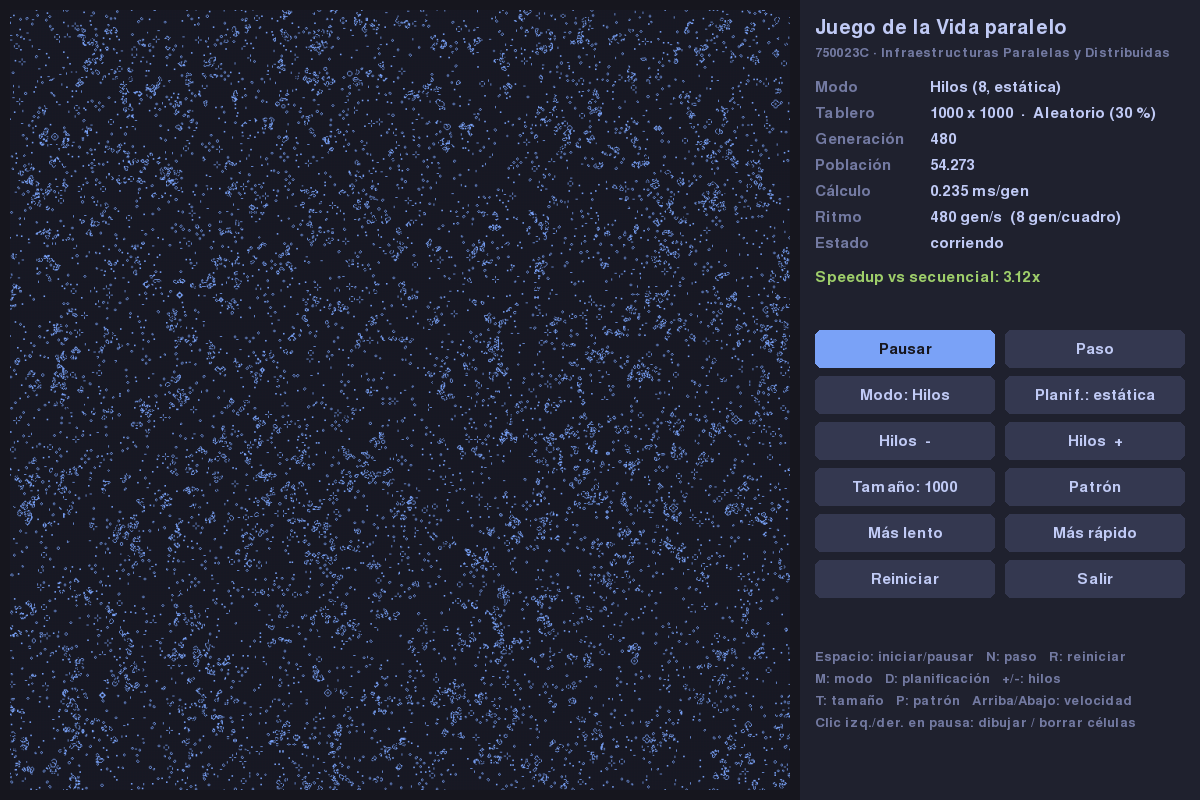
\includegraphics[width=\linewidth]{gui_hilos_1000.png}\caption{Hilos, 1000\x1000.}\end{subfigure}\hfill
\begin{subfigure}{0.49\textwidth}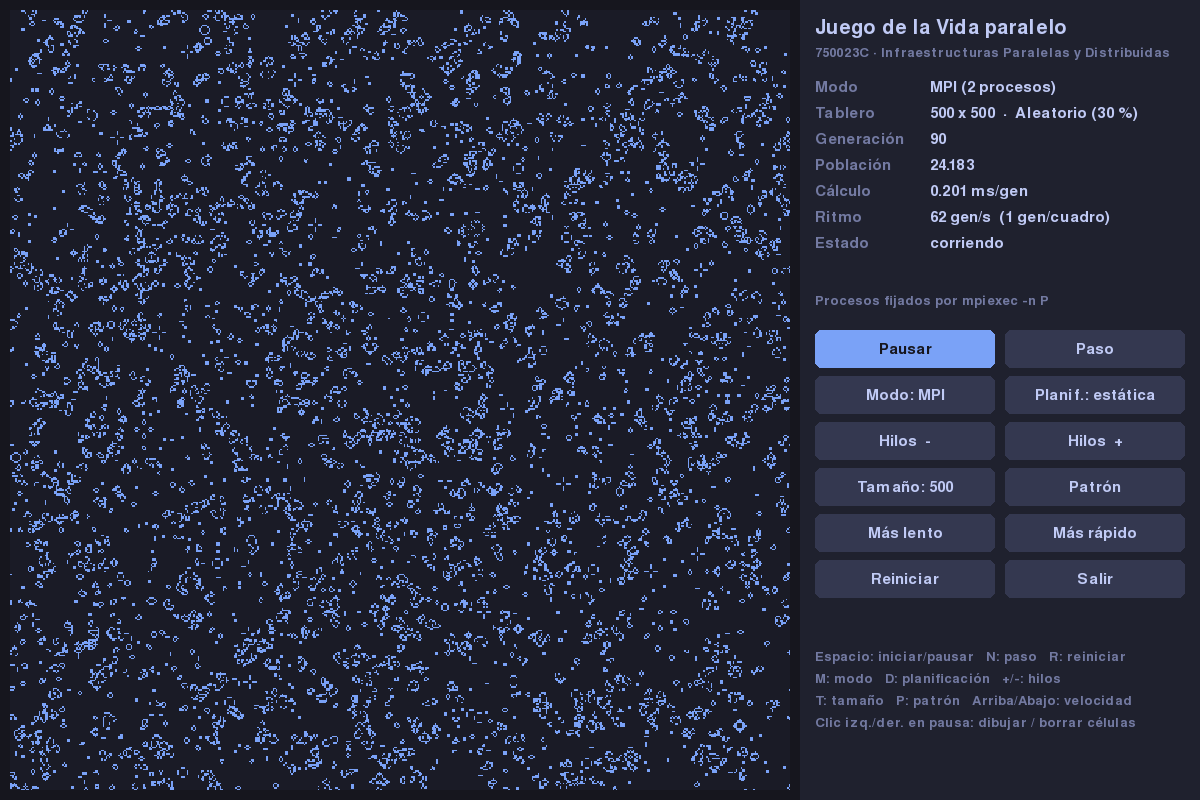
\includegraphics[width=\linewidth]{gui_mpi_500.png}\caption{MPI con 2 procesos, 500\x500.}\end{subfigure}
\caption{Interfaz gráfica. El panel muestra el tiempo de cálculo por generación y el speedup frente a la última medición secuencial del mismo tamaño.}
\label{fig:gui}
\end{figure}

% =====================================================================
\section{Desafíos encontrados}\label{sec:desafios}

\subsection{El GIL de Python}\label{sec:gil}

En CPython el \emph{Global Interpreter Lock} permite que un solo hilo ejecute código Python a la vez. Si el
kernel es Python puro, los hilos se turnan y no hay aceleración. La figura~\ref{fig:gil} lo muestra con
el mismo motor de hilos y tres kernels distintos sobre un tablero de \dato{gil-n}\x\dato{gil-n}:

\begin{itemize}
  \item \textbf{Python puro}: speedup de \dato{gil-python-2} con 2 hilos y \dato{gil-python-\dato{gil-hmax}} con
        \dato{gil-hmax}. El GIL serializa los hilos.
  \item \textbf{NumPy}: NumPy suelta el GIL dentro de cada operación vectorizada, pero lo retoma entre una y otra,
        así que hay paralelismo parcial (\dato{gil-numpy-2} con 2 hilos).
  \item \textbf{Numba con \code{nogil=True}}: el kernel completo corre sin el GIL (\dato{gil-numba-2} con 2 hilos).
\end{itemize}

\begin{figure}[H]
\centering
\begin{minipage}{0.49\textwidth}\centering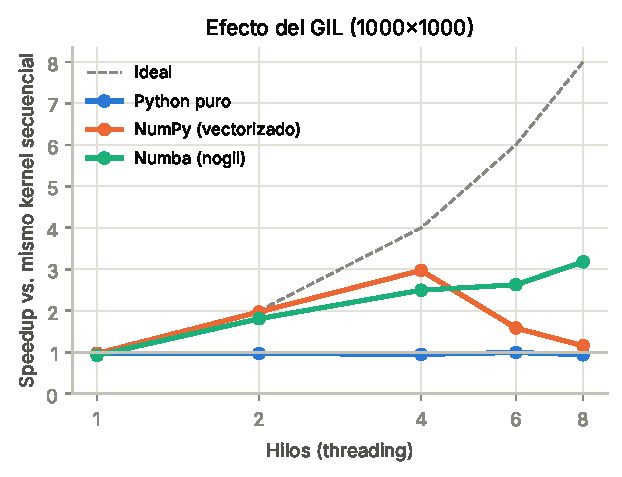
\includegraphics[width=\linewidth]{gil.pdf}
\captionof{figure}{Speedup de la versión con hilos según el kernel.}\label{fig:gil}\end{minipage}\hfill
\begin{minipage}{0.49\textwidth}\centering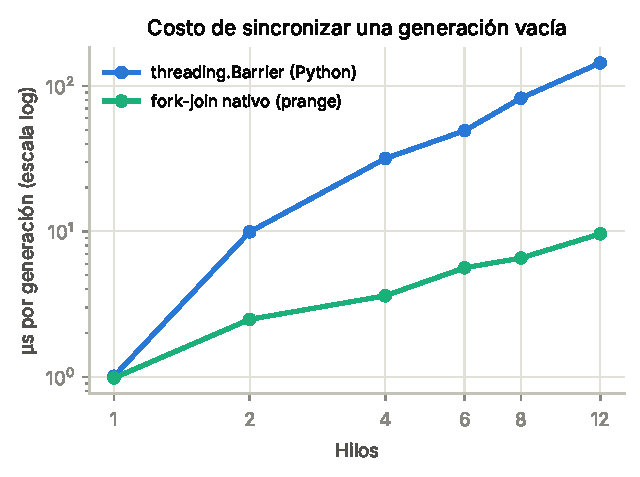
\includegraphics[width=\linewidth]{sincronizacion.pdf}
\captionof{figure}{Costo de sincronizar una generación sin cálculo.}\label{fig:sinc}\end{minipage}
\end{figure}

Por eso todas las versiones usan el kernel de Numba. Una alternativa habría sido usar procesos
(\code{multiprocessing}) con memoria compartida; la versión MPI ya cubre el modelo de procesos.
Desde Python 3.13 existe una compilación experimental \emph{sin GIL} (\emph{free-threaded}, PEP~703)
en la que incluso el kernel de Python puro escalaría con hilos.

\subsection{Condiciones de carrera y la necesidad de la barrera}\label{sec:carrera}

Para comprobar que la sincronización es necesaria, el script \code{bench/demo\_condicion\_carrera.py} ejecuta
\dato{carr-gens} generaciones de un tablero de \dato{carr-n}\x\dato{carr-n} con \dato{carr-hilos} hilos en tres variantes
y cuenta las células que difieren del resultado secuencial:

\begin{itemize}
  \item \textbf{Sin barrera entre generaciones}: un hilo que termina rápido empieza la generación siguiente
        leyendo las filas de frontera de su vecino, que todavía no las ha actualizado. Resultado: entre
        \dato{carr-min} y \dato{carr-max} células erróneas, \emph{distintas en cada uno de los \dato{carr-intentos}
        intentos}. Ese no determinismo es la firma de una condición de carrera.
  \item \textbf{Actualización en el mismo arreglo} (sin doble buffer), incluso con un solo hilo: las células
        ya actualizadas contaminan el conteo de sus vecinas. Resultado: \dato{carr-mismo} células erróneas.
  \item \textbf{Versión correcta} (barrera + doble buffer): \dato{carr-ok} células distintas en todos los intentos.
\end{itemize}

\subsection{Granularidad: el costo fijo de sincronizar}

Cada generación paga una barrera, sin importar el tamaño del tablero. La figura~\ref{fig:sinc} mide ese costo con
un kernel vacío: con \code{threading.Barrier} cuesta \dato{sync-py-2}~µs con 2 hilos y \dato{sync-py-\dato{sync-tmax}}~µs
con \dato{sync-tmax}, porque cada espera implica adquirir un lock, una variable de condición y el GIL para
despertar a cada hilo. El fork-join nativo de \code{prange} cuesta \dato{sync-nat-2} y
\dato{sync-nat-\dato{sync-tmax}}~µs respectivamente. Comparado con los \dato{seq-\dato{nmin}}~ms que tarda
una generación secuencial de \dato{nmin}\x\dato{nmin}, \emph{sincronizar cuesta más que calcular}. Este es el
desafío que más influyó en los resultados.

La planificación dinámica agrava el problema en tableros pequeños: los $8P$ bloques implican $8P$ adquisiciones
del lock por generación, cada una con su llamada desde Python.

\subsection{Interbloqueo en el intercambio de MPI}\label{sec:deadlock}

La forma ingenua del intercambio es que cada proceso haga \code{Send} a su vecino y luego \code{Recv}. Si los envíos
son bloqueantes y todos los procesos envían a la vez, todos esperan a que alguien reciba y nadie llega
al \code{Recv}: se cumplen las condiciones de Coffman \cite{ostep} con una espera circular alrededor del anillo.
Que funcione o no depende de si la implementación de MPI almacena el mensaje en un buffer interno (los mensajes
pequeños sí, los grandes no), lo que hace el error intermitente. \code{Sendrecv} resuelve el problema porque
la biblioteca empareja internamente el envío y la recepción.

\subsection{Desbalance de carga}

En la planificación estática el tiempo de cada generación es el del hilo \emph{más lento}: los demás esperan en
la barrera. El motor registra el tiempo de cómputo de cada hilo; la figura~\ref{fig:desbalance} muestra la razón
entre el hilo más lento y el promedio. En CPUs híbridas (núcleos P y E, como las Intel de 12.ª generación en
adelante) o con el sistema operativo moviendo hilos entre núcleos, esta razón crece y la planificación dinámica
compensa.

\subsection{Medir de forma confiable}

\begin{itemize}
  \item La compilación JIT se hace al importar (firma explícita), nunca dentro del tiempo medido.
  \item Se ejecutan 3 generaciones de calentamiento antes de cronometrar.
  \item La creación del pool de hilos y el reparto/recolección de MPI (\code{Scatterv}/\code{Gatherv}) quedan fuera
        del tiempo; la sincronización y el intercambio de fronteras de \emph{cada} generación sí se miden, porque son
        parte del algoritmo.
  \item El número de generaciones se calibra por tamaño (corridas secuenciales de $\approx$0,6\,s) y es el mismo para
        todas las versiones de ese tamaño.
  \item Cada configuración se repite \dato{reps} veces y se reporta la mediana, menos sensible a interferencias que el promedio.
  \item Cada corrida paralela se compara celda por celda con el resultado secuencial.
\end{itemize}

% =====================================================================
\section{Metodología de medición}\label{sec:metodologia}

\begin{table}[H]
\centering\small
\caption{Entorno de medición (generado automáticamente).}\label{tab:hw}
\begin{tabular}{ll}
\toprule
Procesador & \dato{cpu} \\
Memoria & \dato{memoria} \\
Núcleos físicos / lógicos & \dato{nucleos-fis} / \dato{nucleos-log} \\
Sistema operativo & \dato{sistema} \\
Python / NumPy / Numba & \dato{python} / \dato{numpy} / \dato{numba} \\
Biblioteca MPI & \dato{mpi} \\
Tableros & \dato{tamanos} \\
Hilos / procesos ($P$) & \dato{ps} \\
Repeticiones por configuración & \dato{reps} (se reporta la mediana) \\
\bottomrule
\end{tabular}
\end{table}

Métricas: tiempo por generación $T_P$ (ms), \textbf{speedup} $S_P = T_{\text{sec}}/T_P$ y \textbf{eficiencia}
$E_P = S_P/P$. La línea base $T_{\text{sec}}$ es siempre la versión secuencial con el mismo kernel, no la versión
paralela con $P=1$. Por eso el speedup con $P=1$ mide directamente el sobrecosto de cada mecanismo de paralelización.
Todo el proceso es reproducible con \code{python bench/ejecutar\_todo.py}.

% =====================================================================
\section{Resultados}\label{sec:resultados}

\begin{figure}[H]
\centering
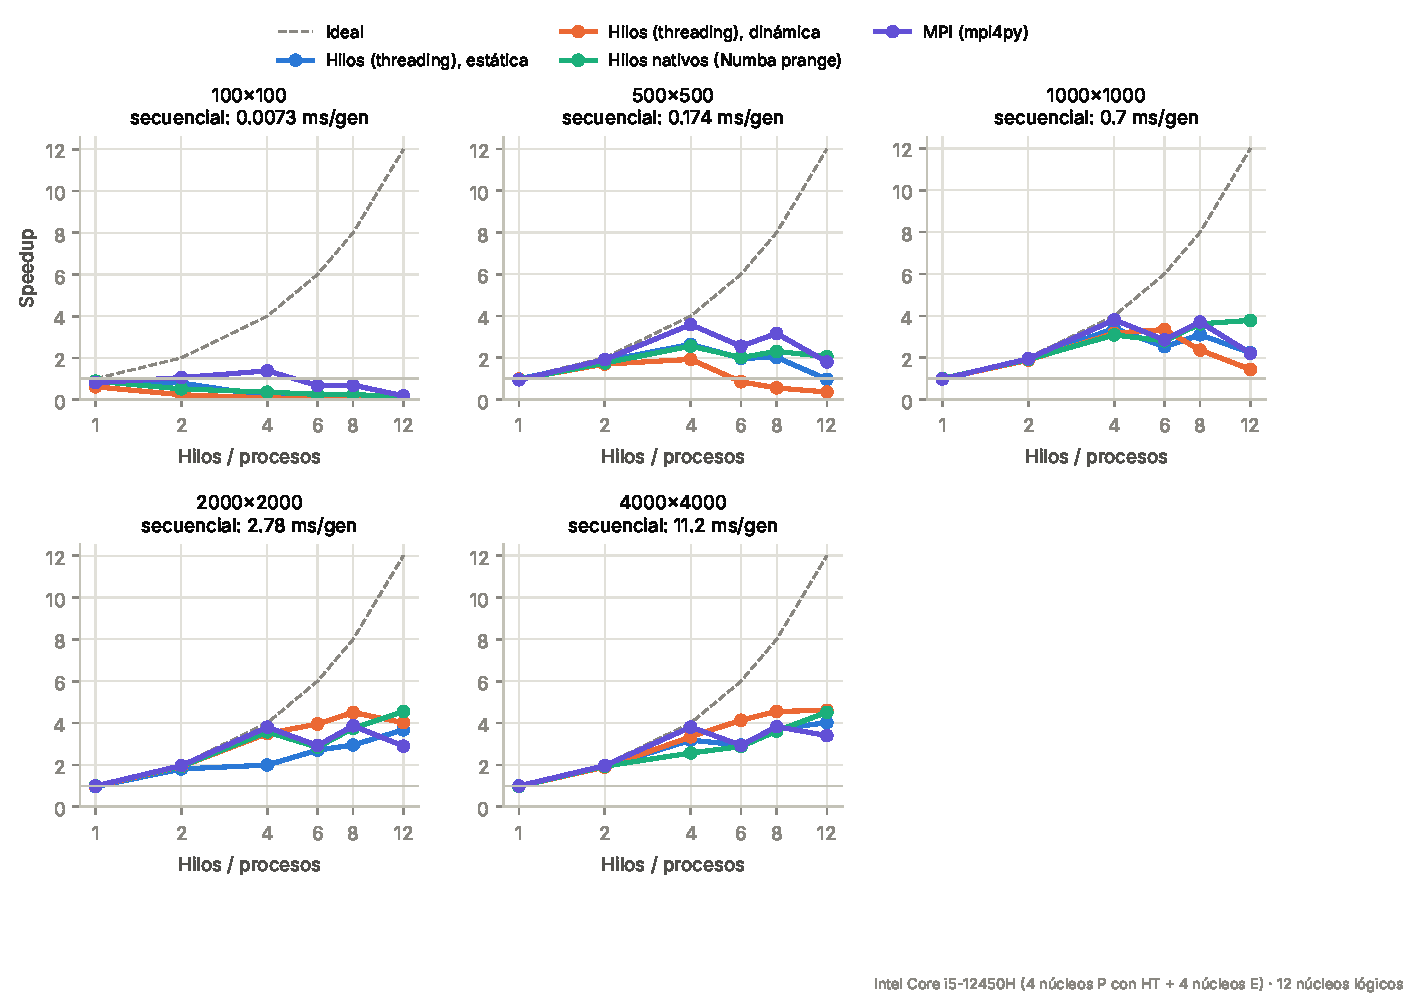
\includegraphics[width=\textwidth]{speedup_por_tamano.pdf}
\caption{Speedup de cada implementación por tamaño de tablero. La línea punteada es el speedup ideal ($S_P=P$).}
\label{fig:sp-tamano}
\end{figure}

\begin{figure}[H]
\centering
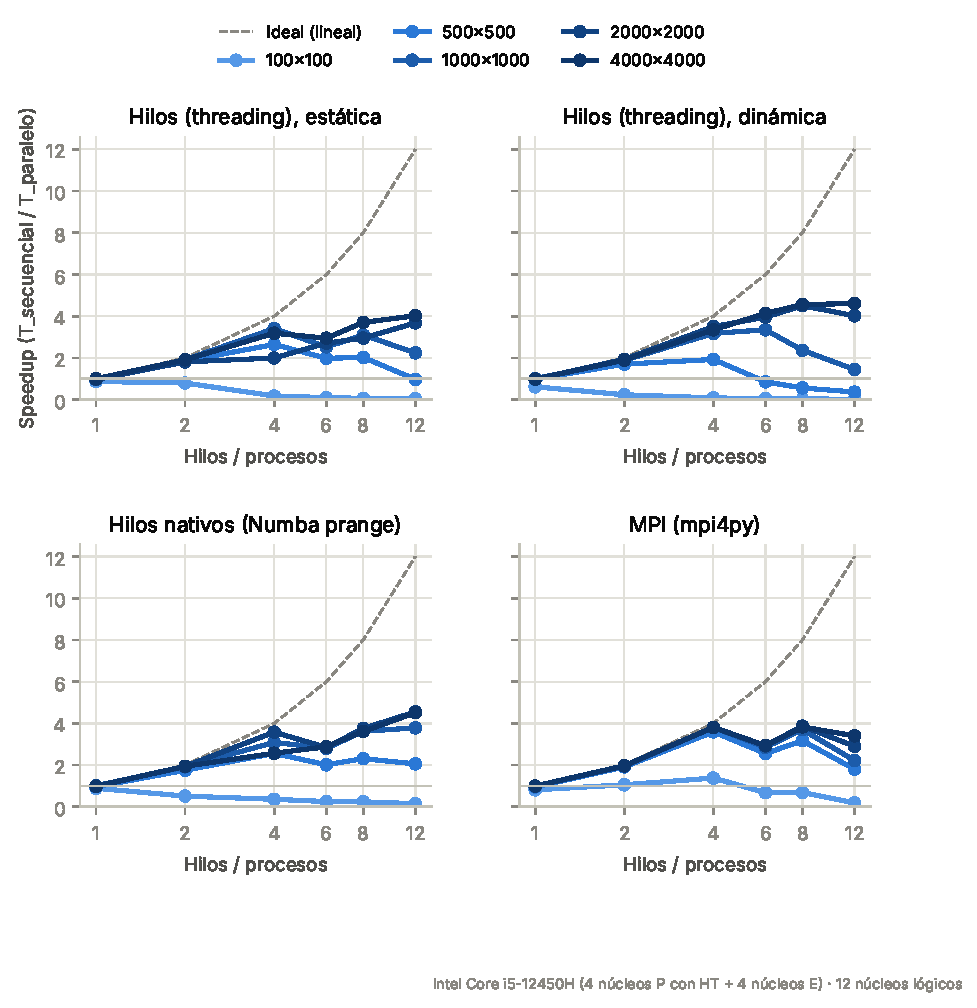
\includegraphics[width=\textwidth]{speedup_por_implementacion.pdf}
\caption{Speedup frente a número de hilos o procesos, con una línea por tamaño de tablero.}
\label{fig:sp-impl}
\end{figure}

\begin{figure}[H]
\centering
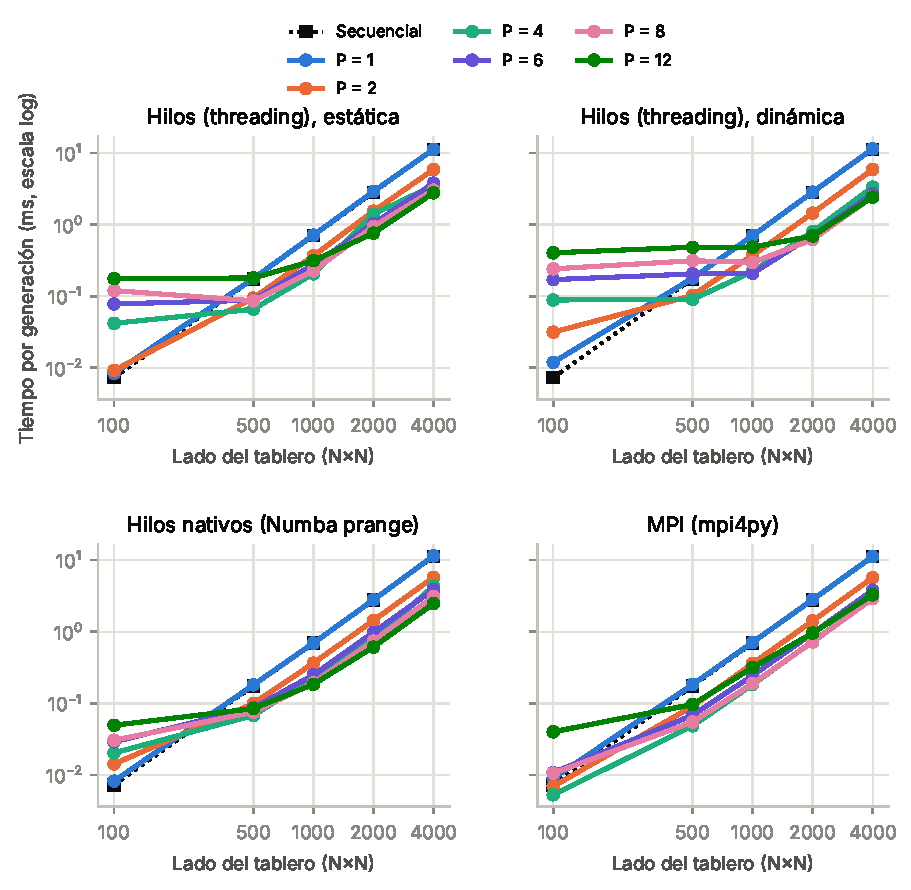
\includegraphics[width=\textwidth]{tiempo_vs_tamano.pdf}
\caption{Tiempo por generación frente al tamaño del tablero (escala logarítmica en ambos ejes).
Con trabajo $O(N^2)$, las curvas deberían ser rectas de pendiente 2; las desviaciones en tableros pequeños
son el costo fijo de sincronizar.}
\label{fig:tiempo}
\end{figure}

\begin{table}[H]
\centering\small
\caption{Speedup (mediana de \dato{reps} repeticiones). En negrita, el mejor valor de cada fila cuando supera 1.}
\label{tab:speedup}
\begin{tabular}{llrrrrrr}
\toprule
Tablero & Implementación & $P=1$ & $P=2$ & $P=4$ & $P=6$ & $P=8$ & $P=12$ \\
\midrule
\multirow{4}{*}{\shortstack[l]{100$\times$100\\\footnotesize sec.: 0,007 ms}} & Hilos, estática & 0,87 & 0,79 & 0,17 & 0,09 & 0,06 & 0,04 \\
 & Hilos, dinámica & 0,61 & 0,23 & 0,08 & 0,04 & 0,03 & 0,02 \\
 & Hilos nativos (prange) & 0,89 & 0,51 & 0,36 & 0,25 & 0,24 & 0,15 \\
 & MPI & 0,81 & 1,05 & \textbf{1,38} & 0,68 & 0,69 & 0,18 \\
\midrule
\multirow{4}{*}{\shortstack[l]{500$\times$500\\\footnotesize sec.: 0,174 ms}} & Hilos, estática & 0,99 & 1,85 & \textbf{2,65} & 1,98 & 2,02 & 0,97 \\
 & Hilos, dinámica & 0,98 & 1,70 & \textbf{1,93} & 0,85 & 0,56 & 0,36 \\
 & Hilos nativos (prange) & 0,96 & 1,75 & \textbf{2,56} & 2,01 & 2,31 & 2,06 \\
 & MPI & 0,95 & 1,91 & \textbf{3,59} & 2,56 & 3,17 & 1,80 \\
\midrule
\multirow{4}{*}{\shortstack[l]{1000$\times$1000\\\footnotesize sec.: 0,700 ms}} & Hilos, estática & 0,98 & 1,91 & \textbf{3,40} & 2,53 & 3,10 & 2,24 \\
 & Hilos, dinámica & 1,00 & 1,88 & 3,17 & \textbf{3,35} & 2,36 & 1,44 \\
 & Hilos nativos (prange) & 1,00 & 1,92 & 3,09 & 2,80 & 3,62 & \textbf{3,79} \\
 & MPI & 0,98 & 1,95 & \textbf{3,81} & 2,85 & 3,70 & 2,21 \\
\midrule
\multirow{4}{*}{\shortstack[l]{2000$\times$2000\\\footnotesize sec.: 2,784 ms}} & Hilos, estática & 0,96 & 1,81 & 1,99 & 2,71 & 2,95 & \textbf{3,68} \\
 & Hilos, dinámica & 0,98 & 1,93 & 3,50 & 3,95 & \textbf{4,50} & 4,02 \\
 & Hilos nativos (prange) & 1,00 & 1,94 & 3,58 & 2,84 & 3,76 & \textbf{4,55} \\
 & MPI & 0,99 & 1,97 & 3,80 & 2,93 & \textbf{3,87} & 2,90 \\
\midrule
\multirow{4}{*}{\shortstack[l]{4000$\times$4000\\\footnotesize sec.: 11,169 ms}} & Hilos, estática & 1,00 & 1,91 & 3,19 & 2,94 & 3,70 & \textbf{4,02} \\
 & Hilos, dinámica & 0,98 & 1,90 & 3,34 & 4,14 & 4,56 & \textbf{4,61} \\
 & Hilos nativos (prange) & 0,98 & 1,94 & 2,57 & 2,88 & 3,62 & \textbf{4,52} \\
 & MPI & 0,99 & 1,97 & 3,81 & 2,94 & \textbf{3,83} & 3,40 \\
\bottomrule
\end{tabular}

\end{table}

\begin{figure}[H]
\centering
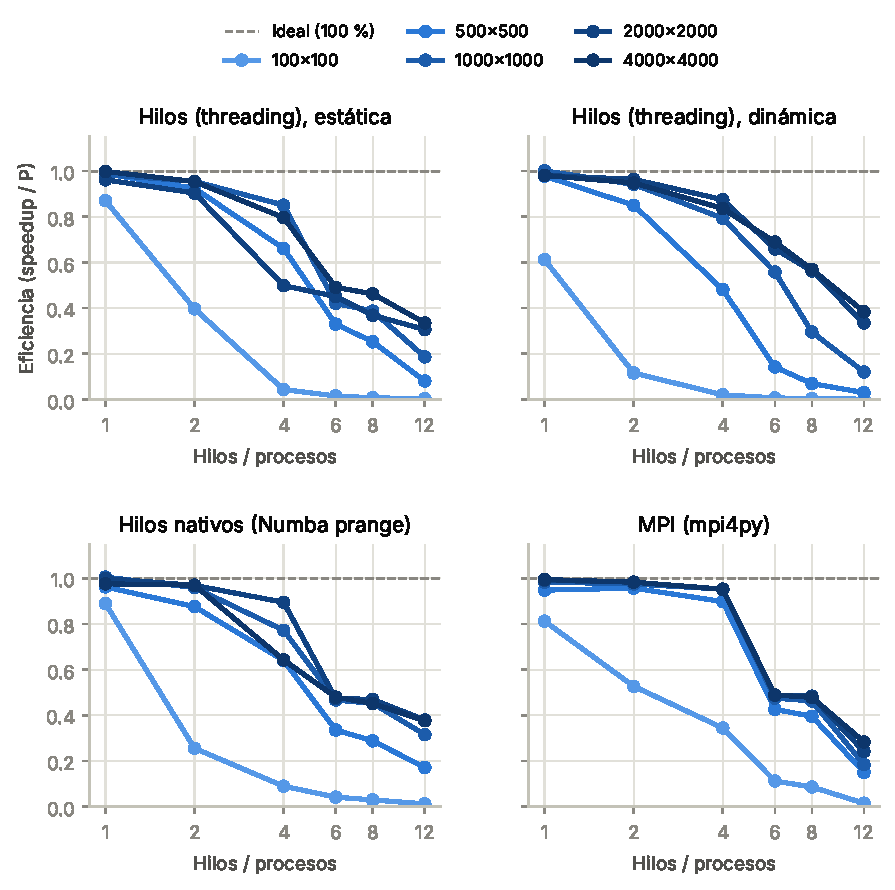
\includegraphics[width=\textwidth]{eficiencia.pdf}
\caption{Eficiencia $E_P = S_P/P$.}
\label{fig:eficiencia}
\end{figure}

\begin{figure}[H]
\centering
\begin{minipage}{0.49\textwidth}\centering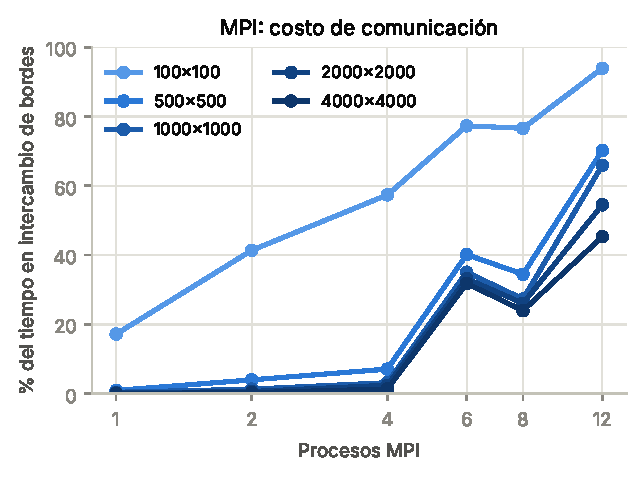
\includegraphics[width=\linewidth]{mpi_comunicacion.pdf}
\captionof{figure}{MPI: porcentaje del tiempo dentro de \code{Sendrecv} (transferencia más espera al vecino).}\label{fig:com}\end{minipage}\hfill
\begin{minipage}{0.49\textwidth}\centering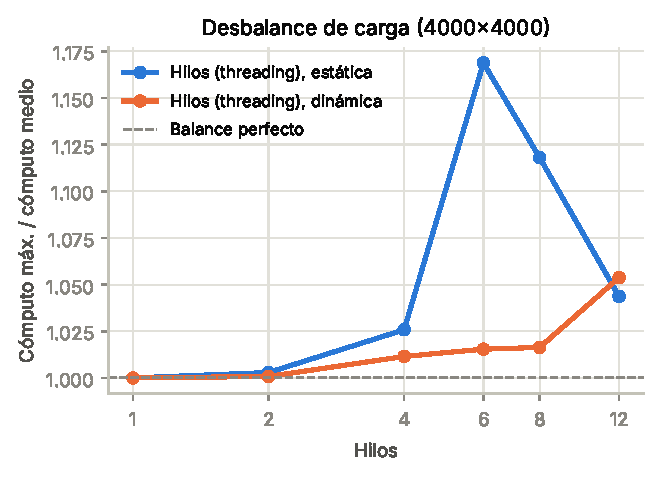
\includegraphics[width=\linewidth]{desbalance.pdf}
\captionof{figure}{Desbalance de carga entre hilos en el tablero más grande.}\label{fig:desbalance}\end{minipage}
\end{figure}

% =====================================================================
\section{Análisis}\label{sec:analisis}

\paragraph{1. El tamaño del tablero decide si el paralelismo vale la pena.}
En \dato{nmin}\x\dato{nmin} una generación secuencial tarda \dato{seq-\dato{nmin}}~ms, del mismo orden que una sola
barrera, así que los hilos son \emph{más lentos} que la versión secuencial (mejor speedup:
\dato{best-hilos_estatica-\dato{nmin}} con \code{threading} y \dato{best-nativo-\dato{nmin}} con hilos nativos).
La única ganancia en ese tamaño fue la de MPI (\dato{bestany-\dato{nmin}}\x{} con $P=\dato{bestany-p-\dato{nmin}}$).
Sus procesos no comparten un GIL, y el \code{Sendrecv} entre procesos de la misma máquina se resuelve en código nativo
sobre memoria compartida, sin pasar por el intérprete. Desde 500\x500 todas las versiones aceleran (mejor:
\dato{bestany-500}\x{}, \dato{bestany-impl-500}, $P=\dato{bestany-p-500}$), porque el trabajo por generación crece como
$N^2$ mientras que el costo de sincronizar se mantiene casi constante. Es lo que anticipa la razón $N/2P$ de la
sección~\ref{sec:estrategia}.

\paragraph{2. La CPU híbrida explica la caída en $P=6$.}
Todas las curvas de speedup suben casi linealmente hasta $P=4$ y \emph{caen} en $P=6$. Por ejemplo, en 1000\x1000
MPI pasa de \dato{sp-mpi-1000-4} a \dato{sp-mpi-1000-6}, y los hilos con planificación estática de
\dato{sp-hilos_estatica-1000-4} a \dato{sp-hilos_estatica-1000-6}. El procesador (\dato{cpu}) tiene 4 núcleos de
rendimiento (P) y 4 de eficiencia (E), más lentos. Con $P\le4$ el sistema operativo ubica a cada trabajador en un
núcleo P. Con $P=6$, algunos trabajadores caen en núcleos E o comparten un núcleo P mediante \emph{hyper-threading}.
Con la partición estática todos reciben la misma cantidad de filas, y en cada generación todos esperan al más lento.
Las mediciones lo confirman:
\begin{itemize}
  \item En MPI, el tiempo de \emph{cómputo} del proceso más lento respecto al promedio sube de
        \dato{desb-mpi-1000-4} con $P=4$ a \dato{desb-mpi-1000-6} con $P=6$.
  \item La fracción del tiempo que los procesos pasan dentro de \code{Sendrecv} (esperando al vecino lento) salta de
        \dato{com-1000-4}\,\% a \dato{com-1000-6}\,\%.
\end{itemize}
La \textbf{planificación dinámica} corrige justamente esto: los núcleos rápidos toman más bloques. En $P=6$ logra
\dato{sp-hilos_dinamica-2000-6} frente a \dato{sp-hilos_estatica-2000-6} de la estática en 2000\x2000, y
\dato{sp-hilos_dinamica-4000-6} frente a \dato{sp-hilos_estatica-4000-6} en \dato{nmax}\x\dato{nmax}. El mejor resultado
de todo el trabajo (\dato{mejor-sp}\x{}) es de la planificación dinámica con \dato{mejor-p} hilos. En tableros pequeños
pasa lo contrario: los $8P$ bloques implican más adquisiciones del lock que trabajo útil, y la dinámica es la peor opción.

\paragraph{3. Un modelo simple explica el comportamiento de \code{threading}.}
Si se suma al tiempo ideal el costo de sincronización medido aparte, $T_P \approx T_{\text{sec}}/P + s(P)$, para
\dato{pred-n}\x\dato{pred-n} con $P=4$ el speedup predicho es \dato{pred4-sp}
($T_{\text{sec}}/4=\dato{pred4-ideal-ms}$~ms más $s(4)=\dato{sync-py-4}$~µs), frente a \dato{pred4-real} medido. Con
núcleos homogéneos, toda la diferencia con el ideal es el costo de la barrera. Con $P=\dato{sync-tmax}$ el mismo modelo
predice \dato{predmax-sp}, pero se midió \dato{predmax-real}. La diferencia restante es la heterogeneidad de núcleos
del punto anterior, que el modelo no incluye.

\paragraph{4. Hilos nativos frente a \code{threading}.}
Las dos versiones usan la misma partición y el mismo kernel; solo cambia quién sincroniza. En este equipo una barrera de
\code{threading} cuesta \dato{sync-py-2}~µs con 2 hilos, pero \dato{sync-py-\dato{sync-tmax}}~µs con
\dato{sync-tmax}, unas \dato{sync-razon} veces más que el fork-join nativo (\dato{sync-nat-\dato{sync-tmax}}~µs).
Con pocos hilos la diferencia casi no se nota (en 500\x500 con $P=4$: \dato{sp-hilos_estatica-500-4} frente a
\dato{sp-nativo-500-4}). Con muchos hilos sí: en 1000\x1000 con $P=\dato{pmax}$, \dato{spmax-nativo-1000} con
hilos nativos frente a \dato{spmax-hilos_estatica-1000} con \code{threading}. El algoritmo escala, y lo que frena a
\code{threading} con muchos hilos es sincronizar desde el intérprete.

\paragraph{5. Ley de Amdahl y fracción serial experimental.}
La ley de Amdahl, $S_P = 1/\big((1-f) + f/P\big)$, acota el speedup según la fracción paralelizable $f$
\cite{pastrana-paralelismo}. A partir del speedup medido se puede estimar la fracción serial \emph{efectiva}
con la métrica de Karp--Flatt \cite{karpflatt},
\[
  e = \frac{1/S_P - 1/P}{1 - 1/P}.
\]
En la tabla~\ref{tab:karp}, para tableros de 1000\x1000 o más y $P\le4$, $e$ queda por debajo de 0,1 en casi todas
las configuraciones (hay dos excepciones aisladas, probablemente por ruido del sistema): el algoritmo es casi
perfectamente paralelizable. En $P=6$, $e$ salta de golpe. Una parte serial real del programa
no puede aparecer de repente al agregar dos trabajadores, así que ese salto no es serialidad sino el sobrecosto de
sincronizar con núcleos de distinta velocidad (punto~2). En los tableros grandes, la planificación dinámica mantiene el
$e$ más bajo para $P\ge6$.

\begin{table}[H]
\centering\small
\caption{Fracción serial efectiva de Karp--Flatt (valores bajos son mejores).}\label{tab:karp}
\begin{tabular}{llrrrrr}
\toprule
Tablero & Implementación & $P=2$ & $P=4$ & $P=6$ & $P=8$ & $P=12$ \\
\midrule
\multirow{4}{*}{500$\times$500} & Hilos, estática & 0,082 & 0,171 & 0,406 & 0,423 & 1,034 \\
 & Hilos, dinámica & 0,176 & 0,359 & 1,208 & 1,906 & 2,928 \\
 & Hilos nativos (prange) & 0,142 & 0,187 & 0,396 & 0,352 & 0,439 \\
 & MPI & 0,045 & 0,038 & 0,269 & 0,218 & 0,514 \\
\midrule
\multirow{4}{*}{1000$\times$1000} & Hilos, estática & 0,047 & 0,058 & 0,275 & 0,226 & 0,396 \\
 & Hilos, dinámica & 0,062 & 0,087 & 0,158 & 0,341 & 0,665 \\
 & Hilos nativos (prange) & 0,043 & 0,098 & 0,228 & 0,173 & 0,197 \\
 & MPI & 0,026 & 0,017 & 0,221 & 0,166 & 0,402 \\
\midrule
\multirow{4}{*}{2000$\times$2000} & Hilos, estática & 0,106 & 0,335 & 0,244 & 0,244 & 0,206 \\
 & Hilos, dinámica & 0,037 & 0,048 & 0,103 & 0,111 & 0,181 \\
 & Hilos nativos (prange) & 0,032 & 0,039 & 0,222 & 0,161 & 0,149 \\
 & MPI & 0,017 & 0,017 & 0,210 & 0,153 & 0,285 \\
\midrule
\multirow{4}{*}{4000$\times$4000} & Hilos, estática & 0,048 & 0,085 & 0,207 & 0,166 & 0,180 \\
 & Hilos, dinámica & 0,055 & 0,065 & 0,090 & 0,108 & 0,146 \\
 & Hilos nativos (prange) & 0,031 & 0,186 & 0,217 & 0,173 & 0,151 \\
 & MPI & 0,017 & 0,017 & 0,209 & 0,156 & 0,230 \\
\bottomrule
\end{tabular}

\end{table}

\paragraph{6. MPI: comunicación frente a cómputo.}
Con núcleos homogéneos ($P\le4$) la comunicación es casi gratis: en \dato{nmax}\x\dato{nmax} con $P=4$ los procesos pasan
el \dato{com-\dato{nmax}-4}\,\% del tiempo en \code{Sendrecv}. Con $P=\dato{pmax}$ ese porcentaje sube a
\dato{com-\dato{nmax}}\,\% (\dato{com-\dato{nmin}}\,\% en \dato{nmin}\x\dato{nmin}; figura~\ref{fig:com}). Ese tiempo
incluye la espera al vecino más lento, así que en este equipo mide sobre todo desbalance y no volumen de datos.
MPI fue la mejor versión con $P=4$ en 500\x500 y 1000\x1000 porque no paga el GIL ni una barrera global: cada
proceso solo espera a sus dos vecinos. Además, es la única versión que podría escalar a varias máquinas sin cambiar el
algoritmo.

\paragraph{7. Memoria y caché.}
Una generación lee un tablero y escribe otro: $2N^2$ bytes. Con $N=4000$ son 32\,MB por generación, bastante más que
los 12\,MB de caché L3 del procesador, así que el kernel queda limitado por el ancho de banda de la RAM
(\dato{memoria}). Aunque 4000\x4000 tiene cuatro veces más trabajo que 2000\x2000, su mejor speedup
(\dato{bestany-4000}) es prácticamente el mismo (\dato{bestany-2000}): agregar hilos no aumenta el ancho de banda de
memoria. Es el ``muro de memoria'' de las arquitecturas multinúcleo visto en clase \cite{pastrana-paralelismo}.

% =====================================================================
\section{Conclusiones}\label{sec:conclusiones}

\begin{enumerate}
  \item \textbf{El paralelismo funciona cuando el trabajo por generación es suficiente.} El mejor resultado fue
        \dato{mejor-sp}\x{} (\dato{mejor-impl}, \dato{mejor-n}\x\dato{mejor-n}, $P=\dato{mejor-p}$). En
        \dato{nmin}\x\dato{nmin} los hilos son más lentos que la versión secuencial, y solo MPI logró una ganancia
        modesta (\dato{bestany-\dato{nmin}}\x).
  \item \textbf{Con núcleos homogéneos el algoritmo escala casi linealmente.} Hasta $P=4$ el speedup está entre 3 y
        3,8 (de un máximo de 4) en casi todas las configuraciones con tableros de 1000\x1000 o más, y la diferencia
        con el ideal se explica casi exactamente por el costo medido de la barrera.
  \item \textbf{En una CPU híbrida, el reparto estático se paga.} Pasar de 4 a 6 trabajadores \emph{reduce} el speedup
        con planificación estática y en MPI, porque todos esperan al núcleo más lento. La planificación dinámica (cola
        de bloques con un lock) recupera ese rendimiento y dio el mejor resultado del trabajo.
  \item \textbf{En Python, los hilos solo sirven si el cálculo suelta el GIL.} Con un kernel en Python puro, los
        hilos no aceleran nada. Con Numba (\code{nogil=True}) sí hay paralelismo real.
  \item \textbf{La corrección depende de dos decisiones}: el doble buffer y la barrera entre generaciones. Sin
        cualquiera de las dos el resultado es incorrecto, y sin la barrera además es no determinista.
  \item \textbf{Hilos frente a MPI.} Los hilos comparten el tablero y no copian datos, pero en Python pagan una
        sincronización cara que crece con el número de hilos. MPI paga dos mensajes por generación y por proceso, pero
        solo sincroniza con sus vecinos y escala a memoria distribuida.
  \item \textbf{Trabajo futuro}: planificación dinámica o reparto proporcional a la velocidad de cada núcleo también
        en MPI; intercambio no bloqueante (\code{Isend}/\code{Irecv}) para solapar la comunicación con el cálculo de
        las filas interiores; filas fantasma más anchas para sincronizar cada $k$ generaciones; y probar Python sin
        GIL (3.13t/3.14t).
\end{enumerate}

% =====================================================================
\appendix
\section{Cómo ejecutar}\label{sec:ejecutar}

\begin{lstlisting}[language=bash]
# Entorno (conda/mamba): incluye MPICH y mpi4py
mamba env create -f environment.yml && mamba activate vida-paralela

python -m vida.gui                                # GUI: secuencial / hilos / nativo
python -m vida.gui --modo hilos --hilos 8 --tamano 1000 --iniciar
mpiexec -n 4 python -m vida.gui_mpi --tamano 1000  # GUI de la versión MPI

python -m pytest -q                                # pruebas de correctitud
python bench/demo_condicion_carrera.py             # demostración sin barrera
python bench/ejecutar_todo.py                      # todas las mediciones y gráficas
python informe/generar_datos.py && cd informe && latexmk -pdf informe.tex
\end{lstlisting}

\section{Tiempos completos}

\begin{table}[H]
\centering\footnotesize
\caption{Tiempo por generación en milisegundos (mediana).}
\begin{tabular}{lrlrrrrrr}
\toprule
Tablero & Gens. & Implementación & $P=1$ & $P=2$ & $P=4$ & $P=6$ & $P=8$ & $P=12$ \\
\midrule
100$\times$100 & 20000 & Secuencial & 0,0073 &  &  &  &  &  \\
 & & Hilos, estática & 0,0084 & 0,0092 & 0,0418 & 0,0779 & 0,1198 & 0,1760 \\
 & & Hilos, dinámica & 0,0119 & 0,0315 & 0,0885 & 0,1704 & 0,2409 & 0,4033 \\
 & & Hilos nativos (prange) & 0,0082 & 0,0143 & 0,0203 & 0,0291 & 0,0306 & 0,0495 \\
 & & MPI & 0,0090 & 0,0069 & 0,0053 & 0,0108 & 0,0106 & 0,0401 \\
\midrule
500$\times$500 & 3514 & Secuencial & 0,1743 &  &  &  &  &  \\
 & & Hilos, estática & 0,1765 & 0,0943 & 0,0659 & 0,0880 & 0,0862 & 0,1797 \\
 & & Hilos, dinámica & 0,1782 & 0,1025 & 0,0905 & 0,2045 & 0,3126 & 0,4823 \\
 & & Hilos nativos (prange) & 0,1812 & 0,0995 & 0,0681 & 0,0866 & 0,0755 & 0,0847 \\
 & & MPI & 0,1839 & 0,0911 & 0,0485 & 0,0682 & 0,0550 & 0,0967 \\
\midrule
1000$\times$1000 & 895 & Secuencial & 0,6998 &  &  &  &  &  \\
 & & Hilos, estática & 0,7111 & 0,3664 & 0,2056 & 0,2771 & 0,2259 & 0,3125 \\
 & & Hilos, dinámica & 0,6991 & 0,3715 & 0,2205 & 0,2090 & 0,2961 & 0,4848 \\
 & & Hilos nativos (prange) & 0,6963 & 0,3648 & 0,2265 & 0,2496 & 0,1934 & 0,1849 \\
 & & MPI & 0,7114 & 0,3589 & 0,1837 & 0,2453 & 0,1889 & 0,3160 \\
\midrule
2000$\times$2000 & 213 & Secuencial & 2,7843 &  &  &  &  &  \\
 & & Hilos, estática & 2,8949 & 1,5402 & 1,3961 & 1,0292 & 0,9434 & 0,7575 \\
 & & Hilos, dinámica & 2,8373 & 1,4443 & 0,7958 & 0,7040 & 0,6182 & 0,6932 \\
 & & Hilos nativos (prange) & 2,7863 & 1,4370 & 0,7779 & 0,9791 & 0,7412 & 0,6117 \\
 & & MPI & 2,8085 & 1,4163 & 0,7319 & 0,9518 & 0,7196 & 0,9601 \\
\midrule
4000$\times$4000 & 53 & Secuencial & 11,1692 &  &  &  &  &  \\
 & & Hilos, estática & 11,1885 & 5,8541 & 3,5067 & 3,7926 & 3,0173 & 2,7768 \\
 & & Hilos, dinámica & 11,3836 & 5,8917 & 3,3398 & 2,7011 & 2,4514 & 2,4235 \\
 & & Hilos nativos (prange) & 11,4455 & 5,7581 & 4,3469 & 3,8800 & 3,0883 & 2,4731 \\
 & & MPI & 11,2330 & 5,6817 & 2,9322 & 3,8040 & 2,9170 & 3,2853 \\
\bottomrule
\end{tabular}

\end{table}

% =====================================================================
\begin{thebibliography}{9}\small
\bibitem{pastrana-tecnicas} M.~A.~Pastrana, \emph{Técnicas de descomposición en algoritmos paralelos}, 750023C, Universidad del Valle, 2026.
\bibitem{pastrana-paralelismo} M.~A.~Pastrana, \emph{Introducción a la programación en paralelo y su importancia en computación}, 750023C, Universidad del Valle, 2026.
\bibitem{pastrana-smp} M.~A.~Pastrana, \emph{Apuntes sobre arquitecturas SMP y SIMD}, 750023C, Universidad del Valle, 2026.
\bibitem{forkjoin} S.~Calvo \emph{et al.}, \emph{Algoritmo paralelo Fork-Join}, exposición, 750023C, Universidad del Valle, 2026.
\bibitem{ostep} R.~H.~Arpaci-Dusseau y A.~C.~Arpaci-Dusseau, \emph{Operating Systems: Three Easy Pieces}, caps.~26--32, 2018.
\bibitem{gardner} M.~Gardner, ``The fantastic combinations of John Conway's new solitaire game `life''', \emph{Scientific American}, 223(4), 1970.
\bibitem{karpflatt} A.~H.~Karp y H.~P.~Flatt, ``Measuring parallel processor performance'', \emph{Communications of the ACM}, 33(5), 1990.
\bibitem{numba} S.~K.~Lam, A.~Pitrou y S.~Seibert, ``Numba: a LLVM-based Python JIT compiler'', \emph{Proc.\ LLVM-HPC}, 2015.
\bibitem{mpi4py} L.~Dalcin y Y.-L.~L.~Fang, ``mpi4py: Status update after 12 years of development'', \emph{Computing in Science \& Engineering}, 23(4), 2021.
\end{thebibliography}

\end{document}
